\pagenumbering{arabic}
\chapter{Background}
\section{Exoplanets}
While we have observed and characterised the planets in our own Solar system for many hundreds of years, the detection of planets orbiting other stars is a relatively new field. The first confirmed exoplanet detection occurred serendipitously, when \citet{1992Wolszczan} observed periodic variations in the timing of the pulses from the pulsar PSR1257+12. Their analysis found that the best explanation for these variations was the presence of two exoplanets with masses 4.3 and 3.9 times the mass of Earth on orbits with semimajor axes 93\% and 119\% of the distance between Mercury and the Sun. Three years later \citet{1995Mayor} found evidence of the first exoplanet orbiting a main sequence star using periodic variations in the radial velocity of the star 51 Pegasi. The exoplanet 51 Pegasi b has a mass 149 times that of Earth and is orbiting at 13\% of the Mercury-Sun distance \citep{2006Butler}.\\ 

Because planets are so much fainter than the stars they orbit, and lie close to those stars on the sky, exoplanetary science almost always uses indirect methods to detect and study these systems. The key properties of an exoplanet that we seek to understand are its mass, composition, and distance from its host star. Exoplanets display a wide range of intrinsic properties such as planetary radius, mass, and atmosphere. While we have used the planets of our Solar system as a template, we cannot be sure that our Solar system is typical. We have found multiple exoplanets with characteristics unlike the planets in our Solar system. For example, the mass of 51 Pegasi b puts it into the Jupiter category, but its orbital radius is 0.0527\,$\pm$\,0.0030 AU, making its surface temperature much hotter than Jupiter itself. Thus 51 Pegasi b became the first known ``hot Jupiter''. Hot Jupiters are more readily detectable to indirect methods than lower-mass planets on longer orbits (see Section\,\ref{secRVPrecision}) and so they formed the majority of discovered exoplanets for a number of years. At first glance this would suggest that close-in gas giants are more common than the ``cold Jupiter'' in our Solar system. However, with the development of exoplanet detection techniques, it has become clear that cold Jupiters are roughly 8 times more common than hot Jupiters \citep{2020Wittenmyer}.\\

In the decades since that first Jupiter-mass planet detection, larger telescopes, higher spectroscopic resolution, improved spectrograph stability, and continued development of data analysis techniques have allowed us to detect smaller and less massive exoplanets. Space-based exoplanet surveys have also played a significant role -- to date, 76\%\footnote{https://exoplanets.nasa.gov/discovery/discoveries-dashboard/} of exoplanets have been detected by space telescopes. Our ultimate goal is to find exoplanets similar to our own planet. Due to our past technological limitations, the fraction of Earth-size exoplanets out of the total number we have detected is relatively low. However, our capabilities are improving, and detection of Earth-sized exoplanets will soon become common.\\

Exoplanet detection requires large volumes of observational data. The probability of detecting exoplanets orbiting any given star is low, while observing time with the most capable telescopes and instruments is limited, so we must optimise by focusing our observations on the stars that are most likely to be hosting the Earth-sized rocky exoplanets we are looking for, and those stars are M-dwarfs.\\

\section{M-dwarfs}
\label{secMdwarfs}
M-dwarfs are the most common type of star in the Galaxy, comprising around 75\% of stars \citep{2007Tarter}. M-dwarfs are the smallest, coolest and least massive stars on the main sequence (Table\,\ref{tabMsub}). Due to the low temperatures of M-dwarf atmospheres, molecules can form that would be destroyed in much hotter stars. Strong absorption features corresponding to titanium oxide (TiO) and vanadium oxide (VO) are observed in optical spectra, while absorption features of carbon monoxide and water are dominant in the near-infrared \citep{2007Tarter,1943Morgan}.\\

\begin{table}[!h]
\centering
\begin{tabular}{| c | c | c | c | c | c | c | c | c | c |}
\hline
SpTy & T & R & Mass & L/100 & M$_{V}$ \\
Dwarf & (K) & (R$_{sun}$) & (M$_{sun}$) & (L$_{sun}$) & (mag) \\
\hline
M0 & 3800 & 0.62 & 0.60 & 7.2 & 9.34 \\
M1 & 3600 & 0.49 & 0.49 & 3.5 & 9.65 \\
M2 & 3400 & 0.44 & 0.44 & 2.3 & 10.12 \\	
M3 & 3250 & 0.39 & 0.36 & 1.5 & 11.15 \\
M4 & 3100 & 0.26 & 0.20 & 0.55 & 12.13 \\	
M5 & 2800 & 0.20 & 0.14 & 0.22 & 16.0 \\
M6 & 2600 & 0.15 & 0.10 & 0.09 & 16.6 \\
M7 & 2500 & 0.12 & ~0.09 & 0.05 & 18.8 \\	
M8 & 2400 & 0.11 & ~0.08 & 0.03 & 19.8 \\
M9 & 2300 & 0.08 & ~0.075 & 0.015 & 17.4 \\
\hline
\end{tabular}
\caption{M-dwarf physical characteristics for each subclass, from \citet{2005Reid}. Note the M4 radius has been altered from 0.36\,R$_{sun}$ to 0.26\,R$_{sun}$, as per \citet{2009Kaltenegger}.}
\label{tabMsub}	
\end{table}

A number of molecular features in M-dwarf spectra vary as a function of temperature and 
luminosity, and have been used as the basis for spectral type classifications that allocate subtypes from warmer (or ``early'') M-dwarfs at M1 to cooler (or ``later'') subtypes at M5-M8. M-dwarf subtype classification was historically complicated by the fact that M-dwarfs emit the majority of their flux in the infrared, and most stellar classification systems had been developed using spectra at optical wavelengths. The most widely adopted spectral classification system currently in use for M-dwarfs was defined by \citet{1991Kirkpatrick}, who based their system on the strengths of TiO and VO absorption bands in the 6300\,-\,9000\,\hbox{\AA} wavelength range. Each individual absorption band tends to grow in strength as we move to cooler stars but then saturate, and so its usefulness as a diagnostic is limited to a certain temperature range. To accommodate this, the \citet{1991Kirkpatrick} classification scheme uses the strength of multiple molecular bands across the wavelength range 6300\,-\,9000 \hbox{\AA} to cover the full range of M-dwarf subtypes. For example, the TiO band at 7050\,\hbox{\AA} can be used for classification of subclasses M0-M5 \citep{2005Reid}, but from M6 onwards the TiO band strength saturates and the classification depends on VO bands. Metal hydrides such as MgH, FeH, and CaH appear weakly in early M-dwarfs and gain strength in later subtypes \citep{2005Reid}. Example spectra from the \citet{1991Kirkpatrick} classification scheme, with important features marked, are shown in Figure~\ref{figMD_sub}.\\

\begin{figure}
\centering
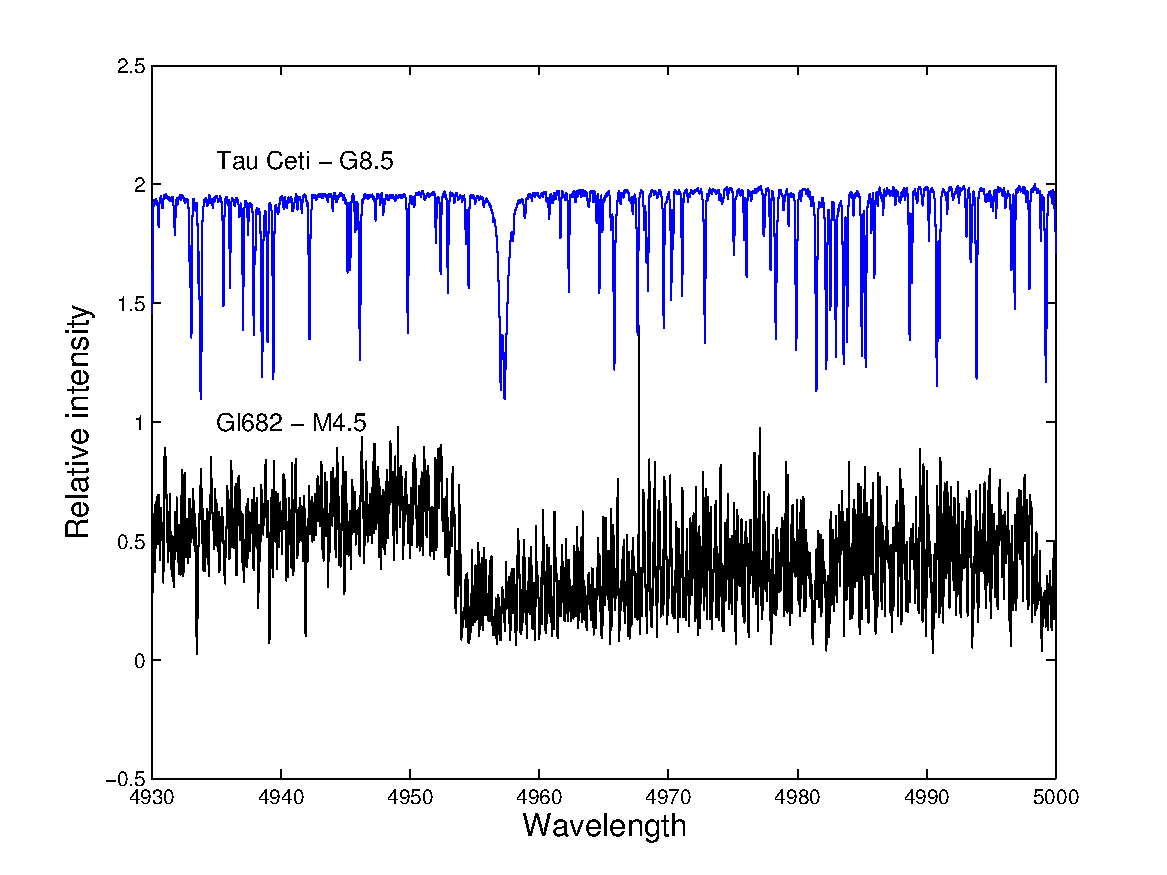
\includegraphics[width=\textwidth]{TauCetiGl682_comparison.pdf}
\caption{Spectra of a G4.5 star, Tau Ceti, and a M8.5 star, Gl682. The spectra have been offset vertically to provide visual clarity. Of note is the molecular bandhead present in the spectra of Gl682 at $\sim$4955\,\hbox{\AA}.}
\label{figSpec}
\end{figure}

Molecular bands like these contain a large number of narrow and closely spaced absorption features, due to the large number of rotational and vibrational energy states available to molecules, and their overall effect on a spectrum is a sharp drop in flux at a particular wavelength and a broad zone of absorption stretching to lower or higher energy. An example of a such a molecular band can be seen in Figure \ref{figSpec}, where the sharp drop of a TiO bandhead is located at $\sim$4955\,\hbox{\AA} and the strength of the absorption decreases toward redder wavelengths. The width of molecular absorption bands can make it difficult to reliably locate the continuum in a spectrum. This complicates spectroscopic analysis, including the measurement of band strength indices and activity (see Section\,\ref{secVarQuant}).\\

\begin{figure}
	\captionsetup{width=.8\textwidth}
	\subfloat[]{\label{figMD_sub_1}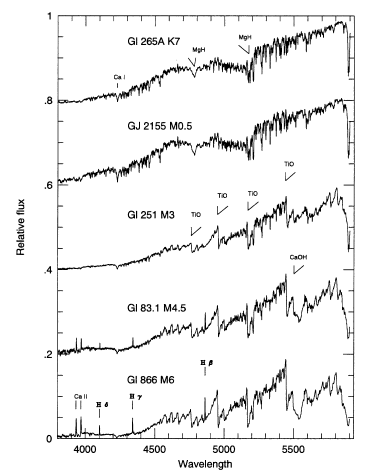
\includegraphics[width=0.52\textwidth]{MD_subclass_1.png}}
    \subfloat[]{\label{figMD_sub_2}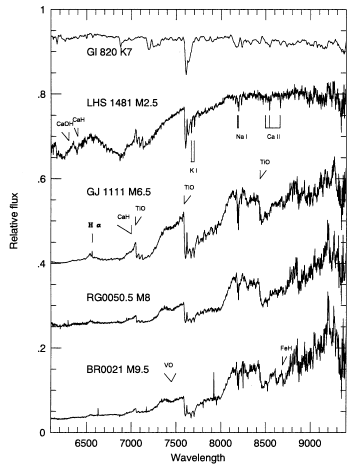
\includegraphics[width=0.5\textwidth]{MD_subclass_2.png}}
    \caption{Spectra of several stars across a range of M-dwarf subclasses and the spectroscopic features used by \citet{1991Kirkpatrick} to classify them. Source: \citet{2005Reid}.}
    \label{figMD_sub}
\end{figure}

\subsection{The habitable zone}
\label{secHab}
Much of current exoplanetary science is motivated by a desire to understand how common potentially habitable planets are in the Universe. One aspect of this is the hunt for observable ``biosignatures'' that could indicate the presence of life. The idea of searching for {\em potentially} habitable exoplanets orbiting in the ``habitable zone'' has become important. The habitable zone of a star is the range of orbital distances at which a rocky exoplanet can retain liquid water at its surface \citep{1993Kasting}. There are multiple parameters that will determine an exoplanet's habitable zone, including its orbital radius, planetary rotation speed, and the mass of the host star. The most significant factor for habitability is the exoplanet's surface temperature, which is primarily dependent on the incident radiation on the exoplanet and therefore on the orbital radius. For a given star system, the location of the habitable zone can vary over time due to the evolution of the star. The habitable zone of the Solar system currently extends from 0.9 to 1.4 AU. Once the Sun ends its hydrogen burning phase, it will evolve into a red giant and the inner boundary of the habitable zone will move outward as the Sun expands, ultimately moving past the Earth. Due to the low luminosity of M-dwarfs, their habitable zones are much closer to the star than for the Sun. Models developed by \citet{2013Kopparapu} predict that a typical M-dwarf habitable zone is 0.2 to 0.8 AU. The fact that the habitable zone for an M-dwarf is quite close to the star makes them important candidates for exoplanet detection, as discussed in Section\,\ref{secTrans}.\\

\section{Exoplanet detection}
\label{secDetectMeth}
Figure\,\ref{figExoHist} shows how the rate of exoplanetary discovery has increased rapidly over time, as the community has continued to develop and improve detection methods. There are a variety of methods that can be used to detect and characterise exoplanets; however, some have been more successful than others. The two methods with the highest yield of planets to date are photometric transits and radial velocity spectroscopy. These two methods allow us to not only detect an exoplanet and determine the parameters of its orbit, but also to estimate its radius (photometric transits) or mass (radial velocity spectroscopy). When both methods can be used together on the same exoplanet, the combined information allows for an estimate of the exoplanet's density and composition.\\

\begin{figure}
    \centering
    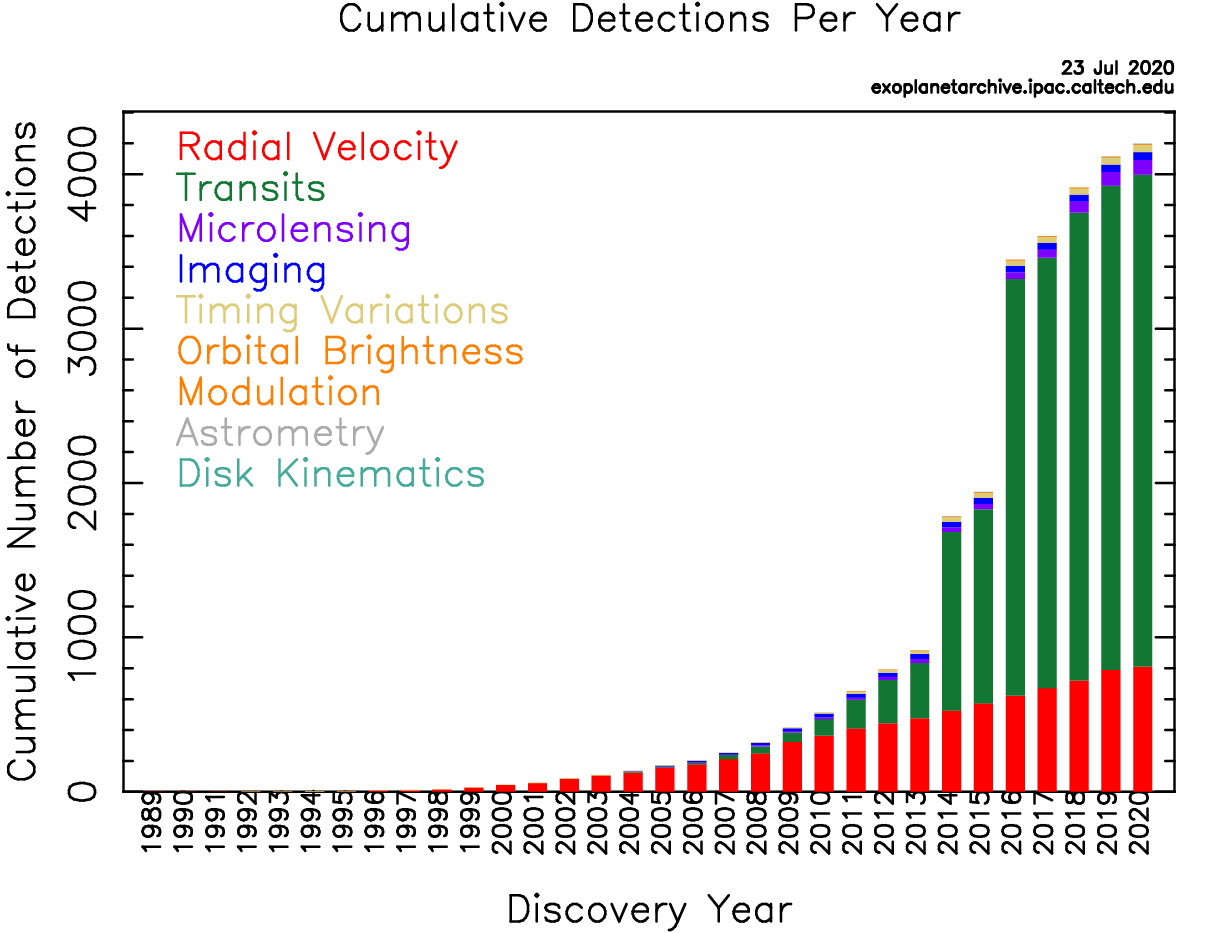
\includegraphics[width=\textwidth]{exo_dischist_cumulative.png}
    \caption{Cumulative histogram of the number of confirmed exoplanets over time. 
    Source: https://exoplanetarchive.ipac.caltech.edu/exoplanetplots/exo\_dischist\_cumulative.png.}
    \label{figExoHist}
\end{figure}

\subsection{Transits}
\label{secTrans}
Transits occur when the path of an exoplanet's orbit aligns with our line of sight to the star. When we observe a transit, the amount of light from the star will change with the position of the exoplanet. Taking Figure\,\ref{figTransit} as an example, when the exoplanet is orbiting outside of the visible disc of the star, the total light we observe is at a maximum. This is the combination of the light from the star and some of the light reflected by the exoplanet. As the exoplanet moves in front of the face of the star, it obscures a small region of the surface of the star, and none of the reflected light is pointing towards Earth. The apparent brightness we observe for the star is at a minimum at this point in the orbit. A smaller secondary dip can be seen when the exoplanet moves behind the star, blocking the reflected light and leaving only the flux directly from the star.\\

\begin{figure}[hbt]
\centering
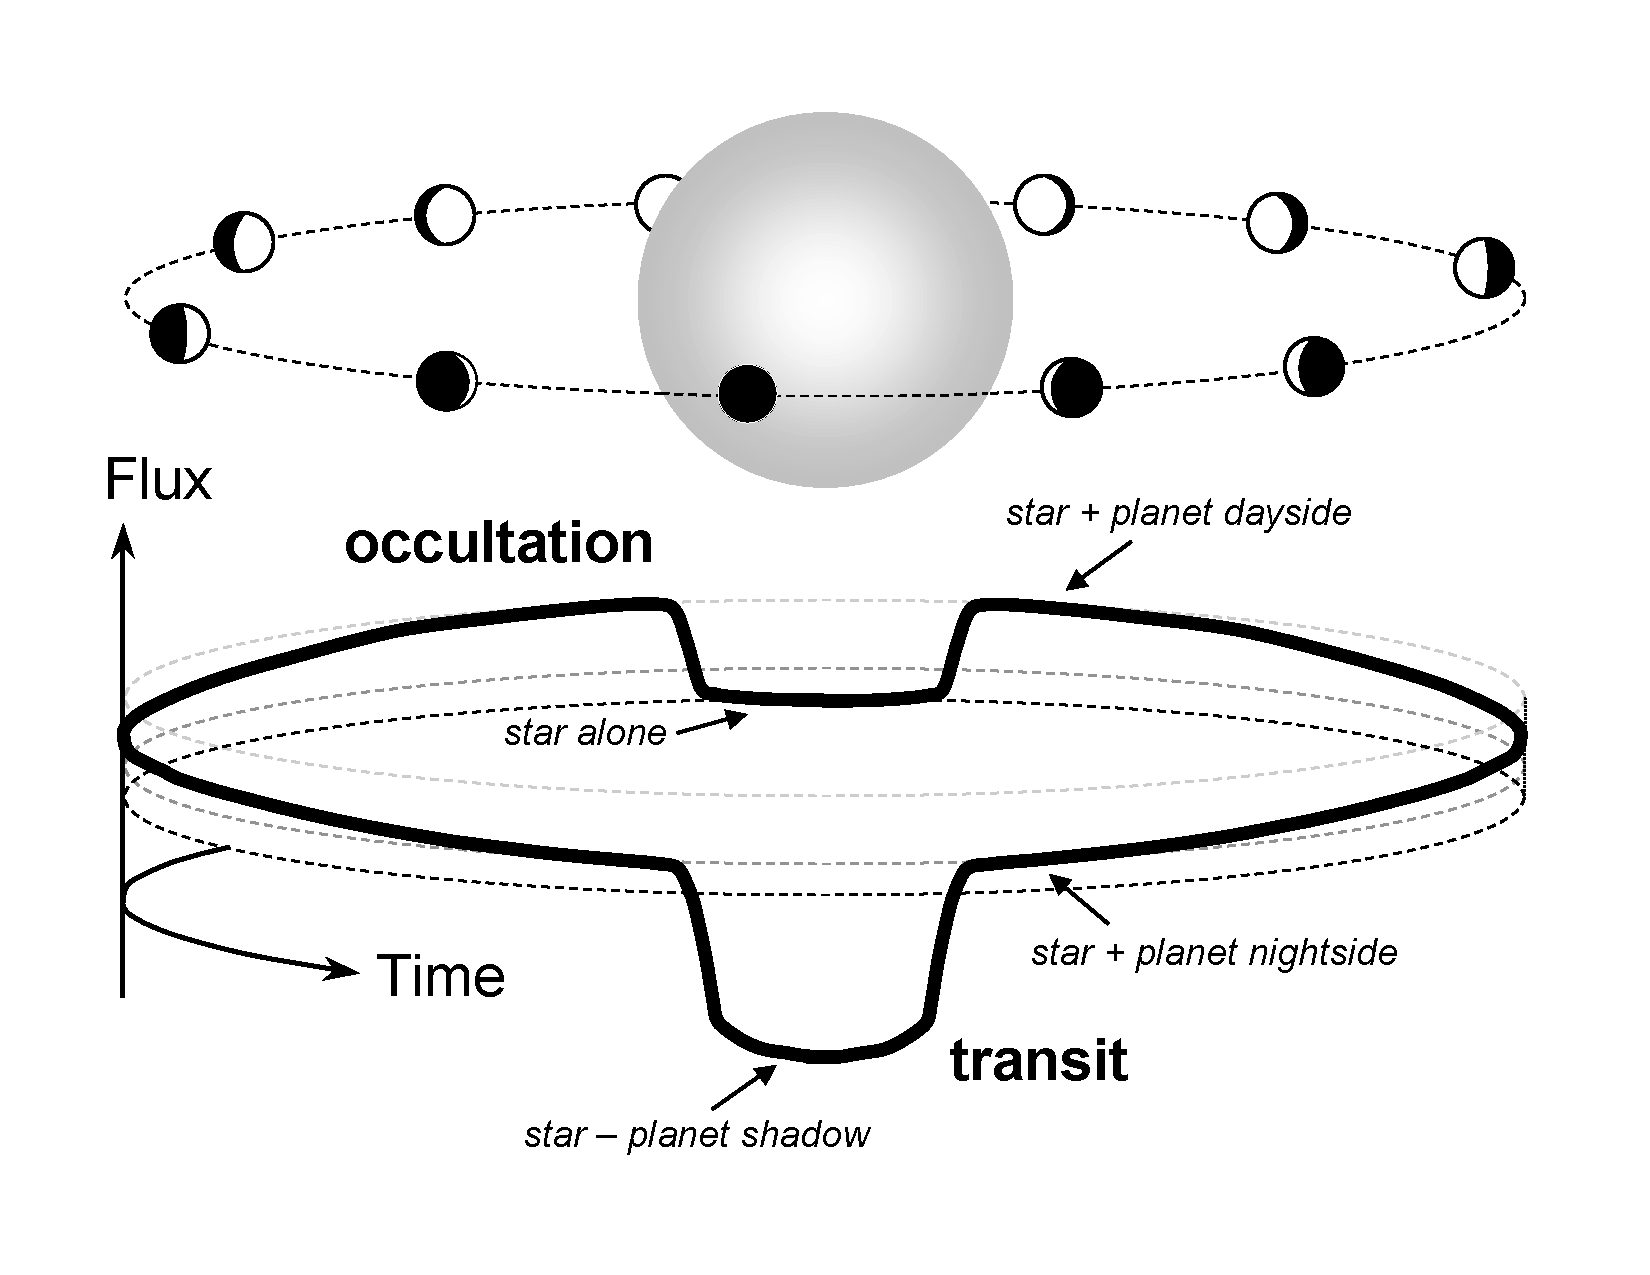
\includegraphics[scale=0.4]{circular_diagram.pdf}
\caption{Diagram showing the effect on the apparent brightness of a star when an exoplanet passes across the visible face of the star. Source: \citet{2010Winn}.}
\label{figTransit}
\end{figure}

We can use this drop in flux to estimate the radius of the exoplanet. Assuming that the stellar disc is uniformly bright, the maximum drop in flux, $\Delta F$, is related to the radii of the exoplanet, $R_p$, and the star, $R_\ast$, through Equation\,\ref{eqFluxDrop}. 

\begin{equation}
\Delta F = \left(\frac{R_p}{R_\ast}\right)^2
\label{eqFluxDrop}
\end{equation}

$\Delta F$ can be determined by a well sampled photometric light curve and $R_\ast$ can be estimated from models of the stellar size as a function of either luminosity (from photometry and distance) or temperature (estimated from photometric colour). In reality the stellar disc is not uniform and limb darkening, where the star is darker at the edges of the disc due to varying optical depth, needs to be taken into account. However, to first order Equation\,\ref{eqFluxDrop} is a reasonable estimate. As an example, if we observed a Jupiter-sized exoplanet transiting a star like the Sun, the drop in flux would be $\sim$1\%. Transit signals in M-dwarfs do not require as much photometric precision as in more massive stars, because the planets are larger relative to the stars, making $\frac{R_p}{R_\ast}$ larger) \citep{2011Lepine}.\\

\begin{figure}
\centering
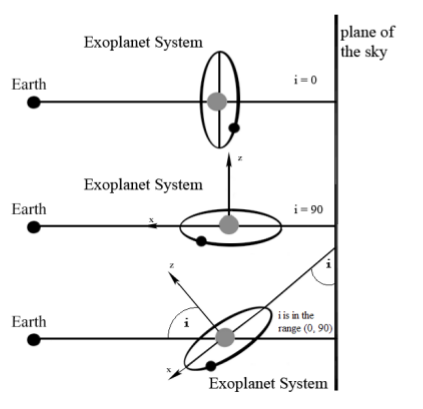
\includegraphics[width=0.7\textwidth]{OrbitalPlane.png}
\caption{Diagram showing the angle representing the orbital inclination of an exoplanet orbiting a star. Source: \citet{1998Zeilik}.}
\label{figOrbit}
\end{figure}

Transits can only be seen if the inclination of the system's orbital plane is close to edge-on ($i \approx 90^\circ$; see Figure\,\ref{figOrbit}). The actual distribution of orbital inclinations will range from $0^\circ$ to $90^\circ$. Assuming randomly distributed orbital orientations and circular orbits, the probability that a given system will have an observable exoplanet transit can be calculated from Equation \ref{eqTransProb}, where $a$ is the semi-major axis of the exoplanet's orbit.\\

\begin{equation}
P_{transit} = \frac{R_\ast + R_p}{a}
\label{eqTransProb}
\end{equation}

For example, if we were observing a star like the Sun, and it had a planet like the Earth, then the probability that the alignment would allow us to see transits would be 0.47\%\citep{2003Borucki}, meaning that we would need to observe approximately 200 of these stars to find one that would transit. Systems containing a large star and/or exoplanet, and those where the exoplanet's orbital radius is small, will have the greatest probability of transiting. Exoplanets orbiting close to their host star, such as habitable zone exoplanets around M-dwarfs, are more likely to have an orbit that allows for the detection of a transit than those on larger orbits. For example, an Earth-sized exoplanet orbiting within the habitable zone of an M7 star (a = 0.35 AU) has a transit probability of $\sim$2.0\%, which is almost four times the transit probability for the same planet orbiting in the habitable zone of the Sun. To accommodate this low geometric transit probability, transit surveys tend to observe large areas of the sky, as their chances of observing a transit increase proportionally with the number of stars observed. The closeness of the habitable zone in M-dwarfs is an advantage to exoplanet detection because of the higher probability of a planet transiting. Planets with smaller orbital radii will have short orbital periods, which allows photometry of multiple orbits to be obtained over a shorter period of time, returning light curves that are well sampled across orbital phase and allowing precise determination of orbital period and transit depth.\\

\subsubsection{Transit surveys}
\label{secTransitSurveys}
There have been a number of ground- and space-based photometric surveys with a focus on exoplanetary transits. The surveys that are of particular importance to this thesis are Kepler, TESS, and the MEarth project. These large survey projects provide photometry in the optical (Kepler) and near-infrared (TESS), which are the wavelengths where M-dwarfs emit most of their flux.\\

The Kepler mission\,\citep{2010Koch} was a spaced-based photometric survey that continuously observed around 150,000 stars across a 115 square degree field of view in an area of the sky around the Cygnus and Lyra constellations. The main aim of continuous photometry of so many stars was the detection of Earth-like exoplanets orbiting in the habitable zone of their star, and the data were also of significant use for studies on asteroseismology \citep{2009Stello} and eclipsing binaries \citep{2006Gimenez}. The survey was initially planned for 3.5 years, starting in 2009, and it was extended to 2016 due to greater than expected stellar variability, which reduced the statistical significance of a transit and resulted in far fewer confirmed transits by Earth-sized exoplanets in the habitable zone than predicted. The Kepler survey team initially estimated they would need three transits per star to get a statistically significant 4\,$\sigma$ light-curve signal-to-noise ratio \citep{2011Gilliland}. However, the variability added noise to the photometric measurements, making additional observations necessary to meet the data quality goals. This extension was interrupted by a technical fault in 2013, when two of the four onboard reaction wheels providing fine pointing control failed. Although Kepler was unable to continue with its initial mission, a ``K2'' mission was developed \citep{2014Howell} in which the spacecraft would observe fields along the ecliptic for 75 days per field. This choice of observing fields allowed the pointing to remain highly stable with only two reaction wheels. The new science goals included observing the transits of nearby low-mass stars (like M-dwarfs), bright stars (V\,\textless\,12), and stars within open clusters, as well as observing star forming regions, type Ia supernovae, and microlensing events. Overall Kepler observed 530,506 stars and detected transits of 2,662 exoplanets across both the original and K2 surveys. An important achievement of Kepler was the discovery of Kepler-22b, the first exoplanet orbiting a Sun-like star in the habitable zone. The planet was found to have a radius of 2.4\,R$_\oplus$ and a mass less than 53\,M$_\oplus$ \citep{2013Kipping}.\\

The Transiting Exoplanet Space Satellite \citep[TESS;][]{2009Ricker} was designed as a followup to the work of the Kepler spacecraft, and it is the current leading source of transiting exoplanet detections, especially around M-dwarfs. Its focus is high quality, high-cadence, wide-field photometry of around 500,000 stars in the Solar neighbourhood, particularly F5-M5 main sequence dwarfs, looking for transiting exoplanets. TESS observes the entire sky, broken into 26 panels of 24 by 96 degrees, with each panel observed for around 27 days. Areas near the ecliptic poles are observed as part of multiple panels, creating a longer time series of data in those regions of sky. Specific targeted stars are observed every 2 minutes, while an image of the full panel is recorded every 30 minutes. Between the observation length and the cadence, TESS transit data focuses on planetary orbits of around 10 days for most stars, and up to 40 or more days for stars near the ecliptic poles.\\

The MEarth project \citep{2008Nutzman} was designed to observe 2,000 nearby (d\,\textless\,33\,pc) M-dwarfs, visible in the northern hemisphere, looking for planetary transits. It is located at the Fred Lawrence Whipple observatory, and uses 8 automated 40cm telescopes. Unlike many current transit surveys, MEarth observes each star sequentially, rather than simultaneously. One of the first major discoveries of the project was GJ1214b \citep{2009Charbonneau}, a 6.55\,M$\oplus$, 2.68\,R$\oplus$ super-Earth orbiting around a star only 13\,pc from Earth. In 2015 an Earth-sized planet was found by the team, orbiting GJ1132 with a radius of 1.2\,R$\oplus$ \citep{2015BertaThompson}. With further analysis, the team determined that GJ1132b had a similar density to Earth, but was orbiting too close to its host star that, while still expected to contain an atmosphere, would not be habitable. Another discovery was a 1.4\,R$\oplus$ planet around LHS1140 \citep{2017Dittmann}. LHS1140b is significant as analysis predicts that the environmental conditions would allow for liquid water to be present on the surface. A second array of MEarth telescopes was built at the Cerro Tololo observatory in Chile \citep{2014BertaThompson}.

\subsection{Radial velocity spectroscopy}
\label{secRVanalysis}
In a planetary system, the star and all the planets orbit their common centre of mass, or barycentre. Figure\,\ref{figOrbit} illustrates this arrangement, and is exaggerated to clearly display that both the star and the planet are moving. Because the star in a real planetary system is much more massive than the planet, the barycentre will be quite close to the centre of the star. 
The more massive the planet is, the further the barycentre will shift away from the centre of mass of the star. As a result, the motion of the star will be small, and so will its velocity, and that velocity signal carries information about the planet's mass and orbit. As an example, the Earth produces a 0.09~ms$^{-1}$ oscillation in the velocity of the Sun with a period of one year, while Jupiter induces a 12.7~ms$^{-1}$ signal with a period of 11.862 years. We can measure the radial velocity of a star from its spectrum by comparing the observed wavelength of a selected spectral line, $\lambda_{obs}$, to its rest wavelength $\lambda_{rest}$. The radial velocity $v_{R}$ is then given by Equation\,\ref{eqRV}, where $c$ is the speed of light.\\

\begin{equation}
    v_{R} = \frac{\lambda_{obs}-\lambda_{rest}}{\lambda_{rest}}c
    \label{eqRV}
\end{equation}

We can improve the precision of this measurement by measuring the shift for many spectral lines simultaneously and combining the results. One common way to achieve this is to cross-correlate the spectrum with a real or synthetic template spectrum with a known radial velocity. A real template spectrum would be taken from observations of a star with the same class as the target star and would often be used in conjunction with a line mask that will restrict the cross-correlation to only the strongest of spectral lines in the spectrum. Synthetic spectra can be  produced by models of a star's atmosphere. One example of this is the PHOENIX code \citep{Phoenix}, which can produce synthetic spectra of stars for a range of temperatures and surface gravities. As long as the star in question and the template star have reasonably similar stellar parameters, the resulting Cross Correlation Function (CCF) is maximised or minimised at the velocity shift required to align the observed spectrum to the template spectrum. Figure\,\ref{figCCF} shows the CCFs for two stars, with the resulting radial velocities marked with vertical dashed lines \citep{2020Morris}. \\

\label{secRV}
\begin{figure}
    \centering
    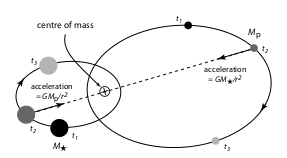
\includegraphics[width=0.8\textwidth]{Barycentre.png}
    \caption{Diagram of a star and a planet orbiting the system's barycentre (labelled as ``centre of mass'' in the diagram). Source: \cite{2011Perryman}.}
    \label{figBary}
\end{figure}

\begin{figure}
    \centering
    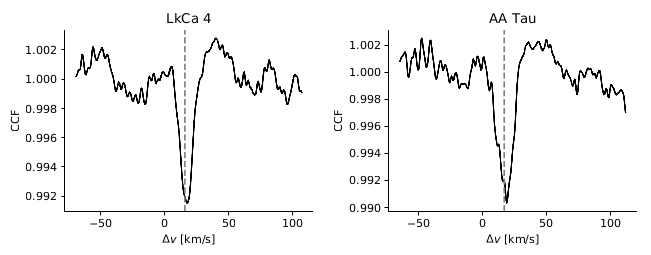
\includegraphics[width=0.8\textwidth]{CCF.png}
    \caption{CCFs for the stars LkCa 4 and AA Tau. The vertical dashed lines mark the radial velocity obtained from the cross-correlation. Source: \citet{2020Morris}.}
    \label{figCCF}
\end{figure}

A radial velocity monitoring campaign for a given star will produce a series of radial velocities. These campaigns are ideally well sampled across multiple planetary orbits to avoid problems with aliasing. We can search for any periodic changes in the radial velocity using least-squares analysis to produce a Lomb-Scargle periodogram \citep{1976Lomb,1982Scargle}. False Alarm Probabilities (FAP) can be calculated to determine how likely it is that a periodogram peak of a given strength was produced solely by noise in the data. The horizontal dotted line in Figure\,\ref{figHD85512Power} represents a 10\% FAP, meaning that noise will produce a peak of that magnitude 10\% of the time. The dashed line is the FAP for 1\%. Assuming an exoplanet's influence on the radial velocity is strong enough, its signal will be prominent in the periodogram and greater than the chosen FAP.\\

\begin{figure}
    \centering
    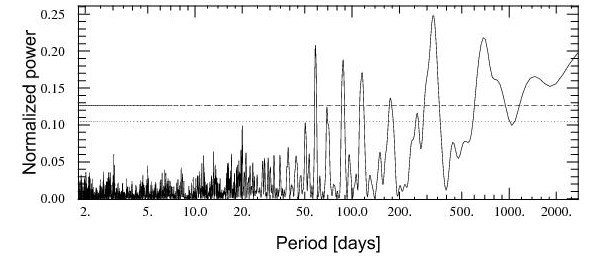
\includegraphics[width=0.8\textwidth]{HD85512_Power.jpg}
    \caption{A periodogram produced from the radial velocities of HD85512. Dashed and dotted horizontal lines indicate FAP of 1\% and 10\% respectively. Source: \citet{2011Pepe}.}
    \label{figHD85512Power}
\end{figure}

For example, \citet{2011Pepe} found several significant peaks in the radial velocity periodogram of HD85512 (Figure\,\ref{figHD85512Power}). A Keplerian model of the radial velocities from a star and planet system was generated from initial estimates of the parameters of the exoplanet (orbital period, eccentricity, planetary mass). The period was selected as each of the peaks of significance in the periodogram and the remaining parameters were varied until the residuals in the radial velocity between the data and the model were minimised. After all the significant peaks were investigated, the influence of an exoplanet with a period of 58.4 days was found in the data (see Figure\,\ref{figHD85512Phased}). The radial velocity signal produced by that planet was removed and a new periodogram, Figure\,\ref{figHD85512Residual}, was produced. In the case of multiple exoplanets, once the first exoplanet is found, its signal is removed from the data, the periodogram is regenerated from the new data, and the process is repeated to see if there are significant and periodic signals remaining in the data. In the HD85512 system, there were no peaks of significance (i.e. above the 1\% and 10\% FAP values) in the periodogram of the residuals, and \citet{2011Pepe} concluded that there were no more planets to be found. Each potential planetary signal needs to be tested against variability measurements to confirm that the signal is not due to a changing stellar environment. Variability is discussed in Sections\,\ref{secVariability}-\ref{secVarQuant} and the impact of variability on HD85512 is detailed in Section\,\ref{secVarApp}.\\

\begin{figure}
    \centering
    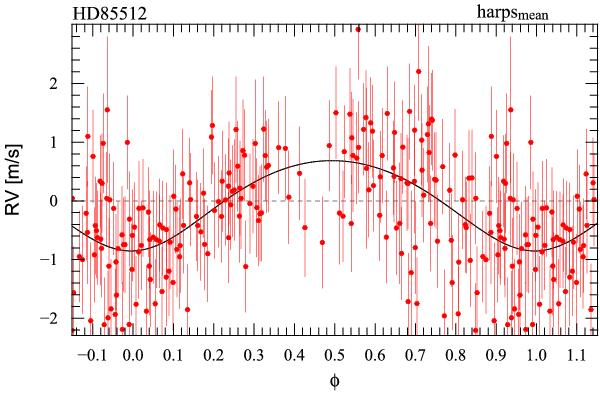
\includegraphics[width=0.8\textwidth]{HD85512_Phased.jpg}
    \caption{Radial velocity for the exoplanet with a orbital period of 58.4 days highlighted in Figure~\ref{figHD85512Periodogram}, as a function of orbital phase $\phi$. The semi-amplitude of the radial velocity variation $K$ is the amplitude of the sinusoid. Source: \citet{2011Pepe}}
    \label{figHD85512Phased}
\end{figure}

\begin{figure}
    \centering
    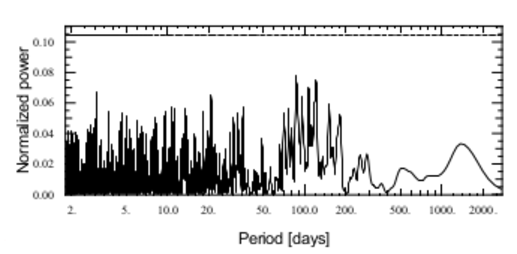
\includegraphics[width=0.8\textwidth]{HD85512_residuals.pdf}
    \caption{Periodogram of the HD85512 radial velocities once the influence of a 58.4 day planet was removed. Source: \citet{2011Pepe}}
    \label{figHD85512Residual}
\end{figure}

Once we know an exoplanet exists, we can determine its mass using the parameters derived from the best-fit model. In Equation \ref{eqRVMass}, $m_p$ is the mass of the exoplanet, $K$ is the semi-amplitude of the radial velocity variation, $G$ is the gravitational constant, $e$ is the orbital eccentricity, $i$ is the orbital inclination (see Figure \ref{figOrbit}), $m_\ast$ is the mass of the star and $a$ is the semi-major axis. The only value we cannot derive from this method is the orbital inclination, $i$. As such, we cannot derive the exact mass of the exoplanet, $m_{p}$, but instead can only determine its minimum mass, $m_{p}\sin(i)$.\\

\begin{equation}
K = \sqrt{\frac{G}{1-e^2}} m_p sin(i) (m_\ast + m_p)^{-1/2} a^{-1/2}
\label{eqRVMass}
\end{equation}

\subsubsection{The influence of spectroscopic precision on radial velocity}
\label{secRVPrecision}
This method has several limitations. First, the radial velocity values we measure are strongly dependent on orbital inclination. We would be unable to detect the movement of stars with orbital inclinations of $0^{\circ}$ (top panel in Figure\,\ref{figOrbit}) and therefore unable to detect the presence of exoplanets by this method. Second, the semi-amplitude of the radial velocity variation, $K$, is dependent on the semi-major axis of the exoplanet's orbit and its mass, in the sense that more massive planets and shorter-period orbits produce larger radial velocity signals. This greater detectability is why hot Jupiters dominated the early days of exoplanet detection. Third, the shape of each spectral line controls how precisely its centroid can be calculated, and therefore how precisely the radial velocity can be calculated. Ideally a spectral line would be narrow, which would allow the centroid of the line to be more accurately determined. There are multiple influences that can broaden a spectral line, and the most influential is the rotation of the star (rotational broadening). \citet{2010Lovis} showed that by assuming a Gaussian profile for a spectral line, the uncertainty $\sigma_{\lambda}$ in the centroid would be proportional to the Full-Width Half-Maximum of the line ($FWHM$) as $\sigma_\lambda \propto FWHM^{\frac{3}{2}}$. M-dwarfs tend to have lower rotational velocities \citep{2005Reid}, so rotational broadening is minimal and the $FWHM$ of a line will be small. \citet{2009Jenkins} studied the rotational velocities of 56 M-dwarfs and found most to be below 10 kms$^{-1}$. A fourth consideration is the number of spectral lines in the observed spectrum, since measuring radial velocity from multiple lines simultaneously leads to a more precise result. The molecular absorption features in the spectra of M-dwarfs create rich forests of lines that are very useful for radial velocity measurement.\\

Perhaps the most important consideration for radial velocity exoplanet detection is velocity precision, which sets a lower mass limit for exoplanet detection. For a confident exoplanet detection, the radial velocity variation amplitude, $K$, needs to be sufficiently larger than the uncertainty associated with each velocity measurement, $\sigma v_{R}$. When the velocity uncertainties are smaller, lower-mass planets are more detectable. The current generation of spectrographs achieve velocity precision of $\sim \pm$1\,ms$^{-1}$, which allows for the detection of small, low-mass, rocky exoplanets in potentially habitable orbits (i.e. exoplanets similar to Earth), which are the priority for current and future exoplanet searches. In the first decade or so of exoplanetary discovery, the best available radial velocity precision was in the $\pm$3-20~ms$^{-1}$ range, permitting the discovery of Jupiter-mass planets on short-period orbits with amplitudes of $\pm$10-100~ms$^{-1}$. Table 2.2 of \citet{2011Perryman} presents a summary of the level of precision achieved by spectrographs in the early years of exoplanet detections. Data for the discovery of 51 Pegasi b \citep{1995Mayor} were acquired with the ELODIE spectrograph \citep{1996Baranne} on the 1.93m telescope at Observatoire de Haute-Provence. The data had a resolution of 42,000, allowing a radial velocity precision of $\pm$\,13\,ms$^{-1}$. The HARPS spectrograph on the 3.6m telescope at La Silla Observatory is a major facility for exoplanet detection. Its maximum spectral resolution is 115,000, which permits a radial velocity precision of $\pm$0.97\,ms$^{-1}$.\\

One of the most important factors in achieving high radial velocity precision is spectrograph stability. When we are trying to measure very small changes in the position of light in the spectrograph that have astrophysical origins, small changes caused by vibrations or changes in atmospheric conditions become significant. For example, with the HARPS spectrograph, the HARPS team identified that the ambient changes in pressure would produce a radial velocity ``drift'' of 100 ms$^{-1}$ per mbar \citep{HARPS}, which is large relative to the radial velocity signal of exoplanets. One mitigation strategy that is used in newer spectrographs is to eliminate moving parts and put the spectrograph into a pressurised tank to control the pressure and temperature. For HARPS, the spectrograph is in an evacuated tank with a pressure below 0.01 mbar. The tank is then air conditioned to ensure that the temperature is maintained at 17\,$\pm$\,0.01$^{\circ}$ C. These measures reduce the radial velocity drift to \textless1 ms$^{-1}$ per day \citealt{2003Mayor}.\\

However, we cannot stabilise our spectrographs completely, and so we also need to measure and correct for these changes. A wavelength calibration, such as Th-Ar hollow cathode lamps \citep{2007Murphy} or a laser frequency comb \citep{1999Reichert}, will produce a spectrum of emission lines that can track the changes in how the spectrograph maps wavelength onto detector position. For most astronomical observations it is sufficient to take wavelength calibration data at the start and end of a night. However, for measurements like radial velocity exoplanet work that require extreme precision, it is necessary to track the wavelength calibration from observation to observation. Light from the calibration lamp or the laser comb is passed through the spectrograph along with the light from the science target, allowing the identification and correction of instrument-based wavelength shifts, making the radial velocity measurement more precise.\\

\subsection{Stellar variability}
\label{secVariability}
While stars are, overall, in hydrostatic equilibrium, they have a non-uniform surface and can rotate at significant velocities that vary with latitude. Their atmospheres are dynamic environments, and there are a number of short-timescale processes that affect the light we receive from them. Rotation, convection, oscillations, temperature variations across the surface, magnetic activity cycles, and other small-scale processes all contribute to an overall ``jitter'' in the radial velocity we measure from a spectrum. Instrumental precision can be improved, but the intrinsic velocity stability of a star is out of our control. The jitter seen in active stars can be large enough that it can be a significant obstacle to our ability to confidently identify the radial velocity signatures of exoplanets. While massive exoplanets can produce a radial velocity variation amplitude large enough to be easily distinguished from the jitter, less massive exoplanets produce radial velocity variations on a similar scale to the jitter, making it harder to confidently identify them.\\

\subsubsection{Stellar atmospheres and magnetic fields}
\label{secStelAtmos}
\begin{figure}
    \centering
    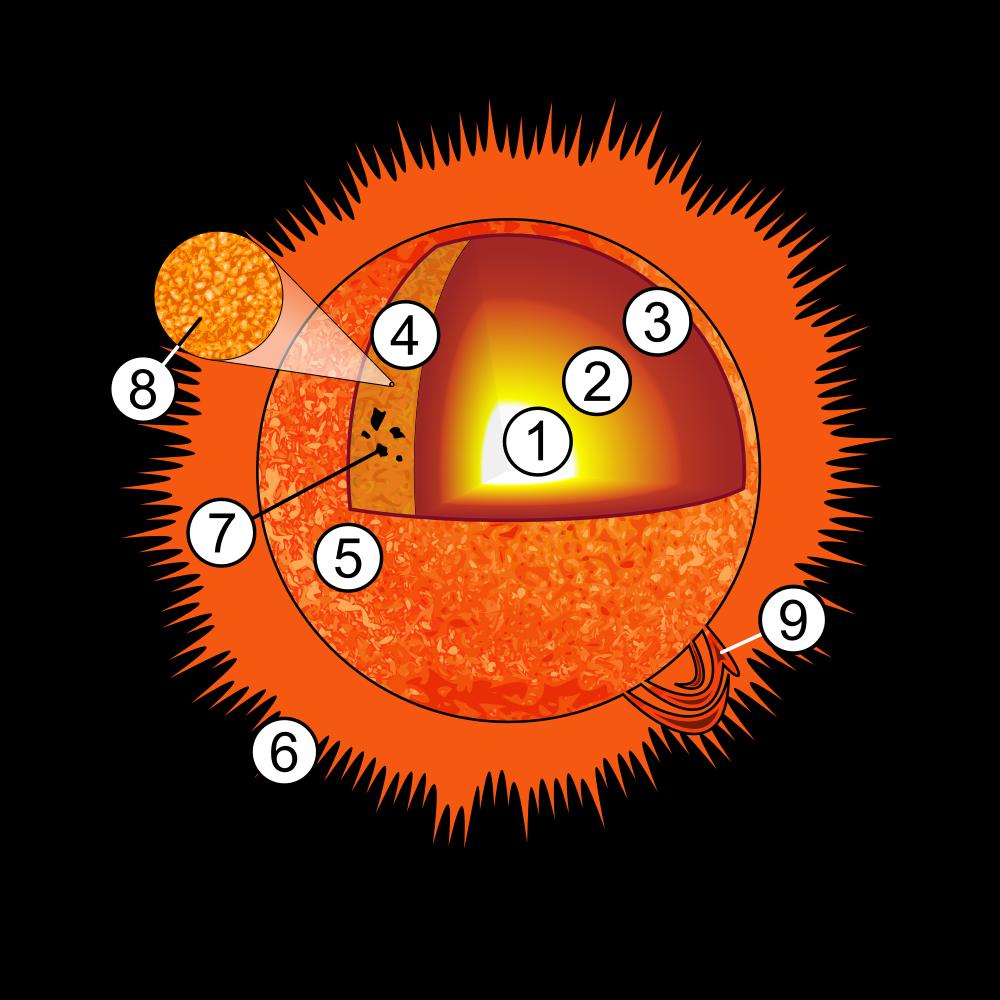
\includegraphics[width=0.6\textwidth]{Sun_diagram.png}
    \caption{Schematic diagram showing the structure of a Sun-like star. The numbered components are:  1. Core, 2. Radiative zone, 3. Convective zone, 4. Photosphere, 5. Chromosphere, 6. Corona, 7. Sunspot, 8. Granules, 9. Prominence. Source: Pbroks13 https://commons.wikimedia.org/wiki/File:Sun\_diagram.svg}
    \label{figStarLayer}
\end{figure}

To understand the astrophysical sources of jitter and their effect on radial velocity measurement, we must consider the structure of the regions that make up the star. Generally, a star has two distinct regions, an opaque interior that produces and transports energy, and a transparent atmosphere that emits the light we see from the star. However, these two regions can then be broken up into additional layers. Figure\,\ref{figStarLayer} labels six layers of a star and three features produced due to stellar magnetic activity. This subsection will discuss the layers of a star, while the following subsection will talk about the stellar activity features.\\

The innermost region of a star is a densely packed region of hot plasma called the core. It is the site of fusion reactions that provide pressure to stabilise the star against gravitational contraction. Outside the core are regions of reduced temperature and density that transport the energy produced by the core to the surface of the star. The structure of these regions, and the methods by which the energy is transported, depend on the mass of the star and the temperature gradient. Energy travelling through a radiative zone is transported as radiation, being absorbed and re-emitted by particles. In a convective zone energy is transported by radiation and mass motion, with hot plasma rising, releasing energy, and sinking back to the base of the convective zone. This cycle produces convective cells, illustrated in Figure\,\ref{figEnergyTrans} as the ellipses in the top layer. Stars more massive than $\approx 2 M_{\odot}$ have convective interiors and radiative exteriors, Sun-like stars have radiative interiors and convective exteriors, and stars with masses \textless0.3\,M$_\odot$ are fully convective and do not have a radiative zone at all. This includes M-dwarfs with types M3.5 and later \citep{2008West}. The details of which regions in a star are stable against convection depend on the opacity and the temperature gradient, with convection only required when the radiation field is not able to transport energy outward as quickly as it is being produced in the core.\\

\begin{figure}
    \centering
    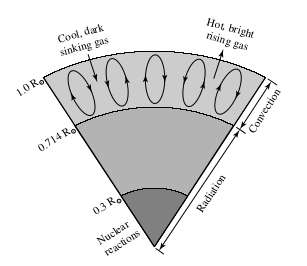
\includegraphics[width=0.6\textwidth]{Convection.png}
    \caption{A schematic diagram of the interior of a Sun-like star. The core produces energy through nuclear fusion, which is then radiated out in the radiative zone. Lastly cells of plasma move in a cycle to transport the energy to the top of the convective zone via convection and convection. Source: \citet{2006Carroll}}
    \label{figEnergyTrans}
\end{figure}

Outside the stellar interior, the first layer of the stellar atmosphere is the photosphere. The photosphere is similar to the convective zone in that there is convective motion present, but is cooler, less dense and is sufficiently transparent for light to have a greater chance of leaving the star and being observed, than of being absorbed. Light moves through the layers of the star in a random walk process, with a mean free path that is dependent on the local density and opacity. The probability of a photon being absorbed and re-emitted is quantified in the optical depth $\tau$, and it is dependent on wavelength and the local sources of opacity. The photosphere of a star is the last scattering surface for photons, which is the depth at which $\tau=2/3$. Since $\tau$ is dependent on wavelength, the depth of the photosphere will vary depending on the wavelength being observed and therefore different spectral features sample the physical conditions at different depths in the star.\\

While the temperature in the stellar interior falls with increasing radius (Figure\,\ref{figSunTempInner}), the layers outward of the photosphere are not so straightforward. The chromosphere is a sparse region situated above the photosphere that opposes the trend of decreasing temperature with increasing radius. The temperature initially decreases in the lower levels of the chromosphere, but then switches and starts to rise, reaching tens of thousands of K at the top (Figure\,\ref{figSunTempOuter}). The reasons for this temperature inversion are complex, and beyond the scope of this work, but essentially it is driven by the presence of magnetic fields in the star \citep{2004Goodman}. Due to this temperature inversion, some elements will produce an absorption line in the cooler regions (the photosphere and lower chromosphere) but also produce an emission line in the upper chromosphere, where the temperature is higher. In particular, the emission from the H$\alpha$ line at 6562.8\,\AA\;and the Calcium H \& K lines at 3968.47\,\AA\;and 3933.66\,\AA\;are quite significant. The outermost layer of a star is the corona. This region extends millions of kilometres into space, and has a temperature of up to 1\,x\,10$^{6}$ K, hot enough to ionise both hydrogen and helium, producing an emission spectrum.\\

\begin{figure}
    \captionsetup{width=.8\textwidth}
    \hspace{-1.5cm}
    \subfloat[]{\label{figSunTempInner}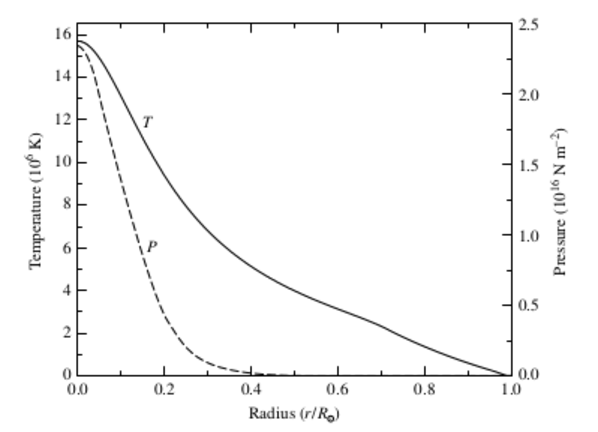
\includegraphics[width=0.6\textwidth]{SunTempInner.pdf}}
    \subfloat[]{\label{figSunTempOuter}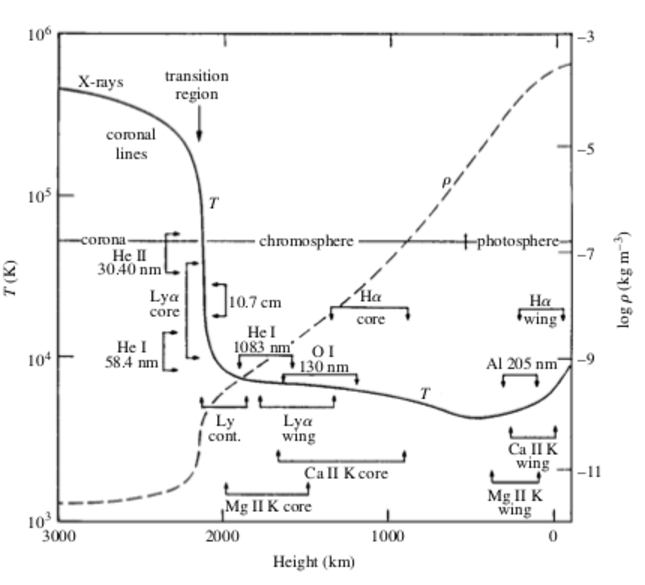
\includegraphics[width=0.6\textwidth]{SunTempOuter.pdf}}
    \caption{Plots of temperature of the interior (left) and atmosphere (right) of the Sun as a function of radius. Source: \citet{2006Carroll}.}
    \label{figSunTemp}
\end{figure}

Threaded through these layers of plasma is a magnetic field formed from stellar rotation and convection within the star, producing a magnetic dynamo. First proposed by \citet{1961Babcock}, dynamo theory states that the motion of charged particles in a star (i.e. the plasma) would induce an electrical current which would in turn induce a magnetic field. Differential rotation of the star will distort the star's magnetic field, twisting the magnetic field lines (shown in panel \textit{b} of Figure\,\ref{figDynamo}), and the interaction of the field lines with the plasma in the star transfers energy from the magnetic field into the stellar atmosphere, heating the chromosphere and producing the stellar activity features discussed in Section\,\ref{secActivity}.\\

In stars with M\,\textgreater\,0.3\,M$_{sun}$, the contrast between the rotation of the interior and the convective zone (solid-body and differential, respectively) produces a region of extreme shear called the tachocline, which will twist the distribution of the magnetic fields across the surface of the star, driving the magnetic dynamo. Stars with M\,\textless\,0.3\,M$_{sun}$ (mid to late M-dwarfs) are fully convective and do not contain a tachocline. The magnetic dynamo of these stars is entirely driven by the differential motion of the convective zone. This will produce significantly stronger magnetic fields than seen in heavier stars, typically 2-5\,kG for active stars \citep{2021Kochukhov}. For comparison, the Sun has a magnetic field of around 1\,G. 

\begin{figure}
    \centering
    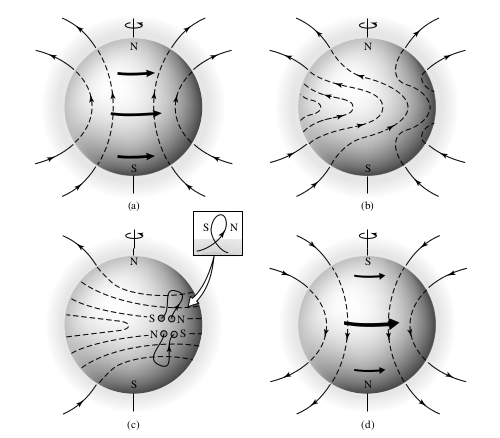
\includegraphics[width=0.8\textwidth]{Dynamo.png}
    \caption{A diagram showing the evolution of a stellar magnetic field. Panel \textit{a} portrays the magnetic field in its initial state, spanning from one pole to the other (poloidal). In panel \textit{b} we see that faster rotation at the equator relative to the poles stretches the field lines across in latitude and the field becomes toroidal. Turbulence from convection will twist the magnetic field into loops that will break through the surface of the photosphere and produce starspots (panel \textit{c}). Eventually the poloidal field will be re-established but with the poles reversed, as seen in panel \textit{d}. Source: \citet{2006Carroll}.}
    \label{figDynamo}
\end{figure}

The magnetic field will go through a cycle of changing magnetic field distribution, from a perfectly longitudinal field from pole to pole (poloidal) to a distorted and predominantly latitudinal field (toroidal) and back again. In the Sun this cycle takes 11 years.\\

\subsubsection{Types of stellar activity}
\label{secActivity}
The features seen on the surface of the Sun are the result of convective motions in the photosphere and chromosphere, and the interaction between the twisted magnetic field of the star and the stellar atmosphere. These features are also seen, to a greater or lesser extent, in almost all stars. These features include granulation, stellar oscillations, starspots, faculae, plages, and flares.\\

\begin{figure}
    \captionsetup{width=.45\textwidth}
    \subfloat[An image of convective granulation on the Sun. Source: https://sdo.gsfc.nasa.gov/assets\newline/img/browse/2010/08/19/\newline20100819\_003221\_4096\_0304.jpg.]{\label{figGranPhot}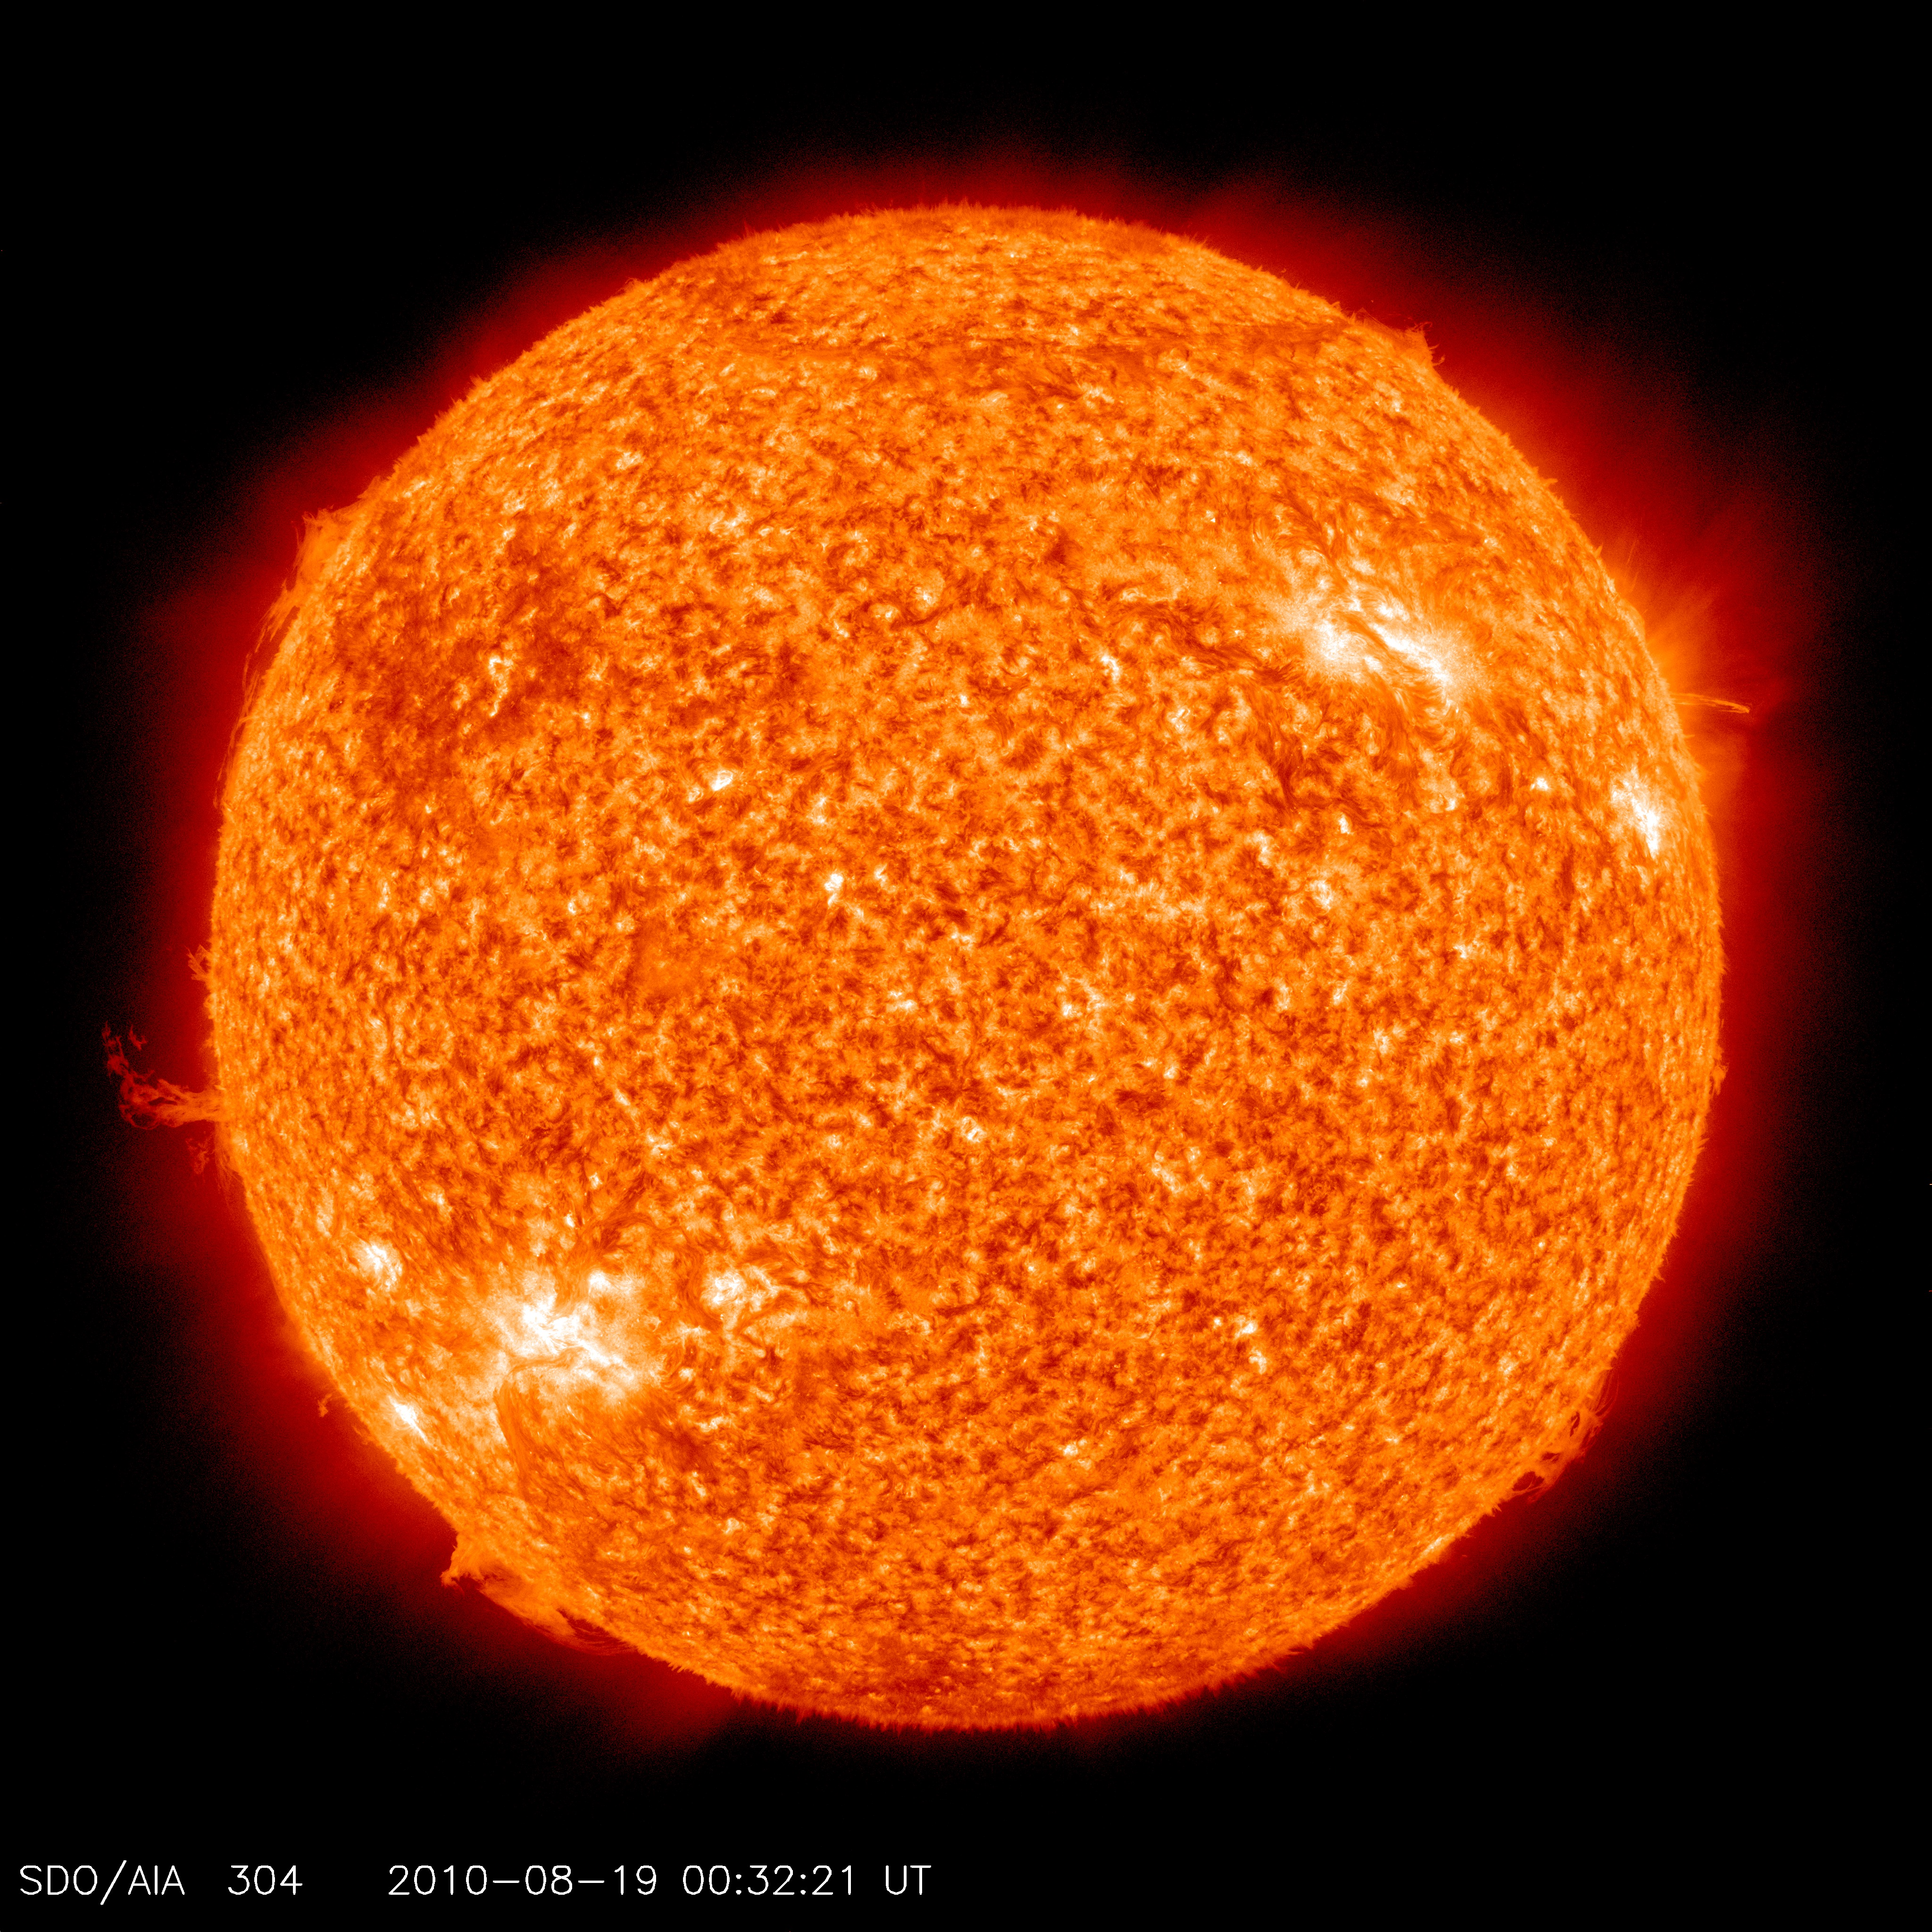
\includegraphics[width=0.5\textwidth]{SunGranulation.jpg}}
    \subfloat[A schematic diagram of convective granulation and how the light from the different parts of the granules are velocity shifted. Source: \citet{2015Haywood}.]{\label{figGranDia}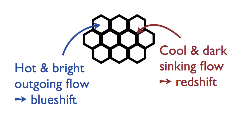
\includegraphics[width=0.5\textwidth]{Granules.png}}
    \caption{}
    \label{figGranSpots}
\end{figure}

Granulation: The convective motion of plasma in the photosphere appears visually as bright and dark cells on the surface of the star (Figure\,\ref{figGranPhot}). This produces blueshifted light in the middle of a granule as the plasma is rising towards the observer, and redshifted light in the intergranular lanes between granules where the plasma is sinking (Figure\,\ref{figGranDia}). In a convective cell there will be the same amount of plasma moving upwards as downwards; however, the rising plasma is hotter and less dense than the sinking plasma. Therefore the granular cells occupy more surface area than the intergranular lanes. The light we see will be the combination of both of these processes and will have a net blueshift. For the Sun this is around 200 ms$^{-1}$ \citep{2010Meunier}. These convective cells of gas range in scale from small (mesogranules) to large (supergranules) with diameters ranging from 150\,km to 2,500\,km and lifetimes from 30 minutes up to a day. \\

Oscillations: Convection is also known to drive acoustic oscillations that move through the star similar to earthquakes in the Earth \citep{1980Cox}. These oscillations were first seen in the Sun \citep{1962Leighton}, and later on observed in other stars. One type, pressure-mode waves\citep{1941Cowling}, travel through the chromosphere, alternating between compressing and expanding the plasma. In the Sun, these oscillations last approximately 5 minutes \citep{1962Leighton}, and are predicted to last from 20-180 minutes in M-dwarfs \citep{2019Rodriguez}.\\

Starspots: Convection will push the magnetic field lines out past the surface of the photosphere into the corona and back down again, producing coronal loops. An illustration of this can be seen in panel \textit{c} of Figure\,\ref{figDynamo}. At the intersection of the coronal loop and the surface of the photosphere we see starspots, which are regions of the surface of a star that are cooler and darker than the surrounding area. Starspots move in position over time as the magnetic field that produced them moves. The concentrated magnetic flux of the loop suppresses convection in the affected area of the photosphere and reduces the surface temperature. The change in temperature can be up to 2000\,K in late F and early G stars and 200\,K for M stars \citep{2009Strassmeier}. Each coronal loop has two points of intersection with the photosphere, and it produces two starspots, one with a north magnetic field and the other with a south magnetic field. As starspots are a byproduct of the magnetic cycle of the star, the number of starspots seen increases as distortion in the magnetic field increases, and will decrease once the polodial magnetic field re-establishes itself. This periodic increase and subsequent decrease in the number of spots is known as the stellar magnetic cycle. One of the earliest investigations of sunspots was by \citealt{1844Schwabe}, while \citealt{1904Maunder} observed that the number of sunspots were at a maximum at mid-latitudes, and decreased as the spots moved towards the equator. For the Sun this cycle has a period of around 11 years, however for M-dwarfs, the magnetic cycle is not only shorter, but also depends on how fast the star is rotating. For fast rotating M-dwarfs (periods of less than a day), the magnetic cycle can last roughly a year, while the slower rotating M-dwarfs have cycles of approximately four years\citep{2019Kuker}. At the maximum of the stellar magnetic cycle, there can be significant numbers of starspots that cover a significant fraction of the visible surface of the star. Early estimates of starspot coverage in cool stars such as M-dwarfs predicted coverage rates of up to 64\%\citep{1995Neff}, however further work has this estimate closer to 40\%\citep{2004Oneal}. Sufficient numbers of starspots will decrease the amount of light coming from the star by a noticeable amount. At the maximum of the solar magnetic cycle, sunspots reduce the light from the Sun by 0.1\% \citep{2006Carroll}.\\

Faculae: Accompanying starspots are regions of the photosphere that appear slightly brighter and hotter (up to 100\,K) than the regular (non-active) regions of the atmosphere. They are most visible at the limbs of the star. Faculae occur in the photosphere as bright points and are often found near starspots, indicating some connection between them, but can also be seen in extended groups independent of a starspot. \citet{1976Spruit} proposed the ``bright wall'' model to explain faculae. Essentially magnetic flux will make the plasma in a convection cell less opaque, allowing a view deeper into the photosphere. Observations of faculae on the Sun by \citet{1978Hiryama} found that faculae can last up to a few hours. One interesting feature of note is that at the time of sunspot maximum, faculae emit enough light to overcome the deficit from the starspots and actually increase the total amount of light seen \citep{2004Keller}.\\

Plages: The chromospheric counterpart to faculae are plages. Plages are larger in scale than faculae and often herald the formation of starspots in a region. They are produced by the interaction of magnetic fields with pockets of plasma that are higher in density than the rest of the chromosphere. Plages can be detected in a spectrum as an emission component, primarily in Ca H \& K and H$\alpha$, and they are the source of H$\alpha$ emission near starspots \citep{2006Carroll}.\\

\begin{figure}
    \captionsetup{width=.45\textwidth}
    \subfloat[A zoomed in photo of the Sun showing starspots (dark regions) with faculae (light regions) surrounding them. Source: https://solarscience.msfc.nasa.gov/feature1.shtml.]{\label{figSunspot}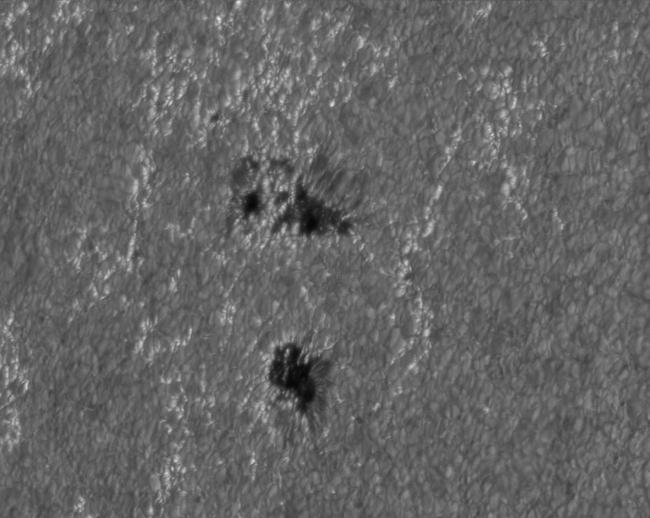
\includegraphics[width=0.555\textwidth]{faculae.jpg}}
    \subfloat[An X-ray image of flares on the surface of the 
    Sun in 2005 from the TRACE satellite. Source: https://www.nasa.gov/mission\_pages/swift/bursts\newline/monster\_flare.html.]{\label{figFlare}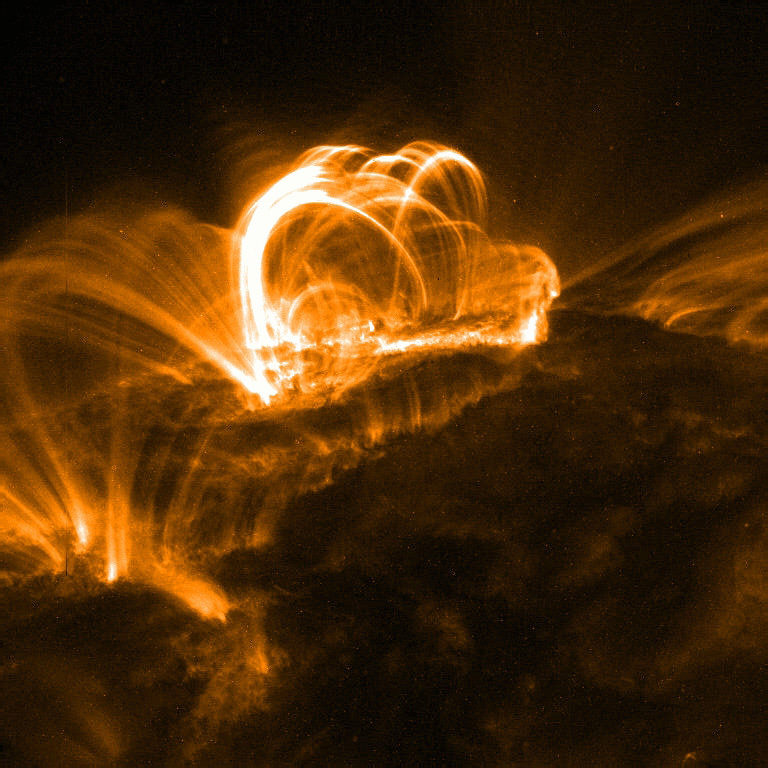
\includegraphics[width=0.445\textwidth]{162169main_Trace_solar_flare_lg.jpg}}
    \caption{}
    \label{figStellActiv}
\end{figure}

Flares: Flares are the result of magnetic reconnection, where the interaction of magnetic field lines converts heat into kinetic energy, producing highly accelerated electrons that will interact with the plasma of a star, resulting in a sudden, but short-lived, release of energy, increasing the brightness of the star by several magnitudes across a wide range of wavelengths \citep{2012Schmidt} and a significant increase in emission line strength. A typical example of the effect of flares on a spectrum is seen in Figure \ref{figFlareDia}. Specific lines in the spectra of EV Lac are significantly stronger while the star is flaring. The black line represents the flux when the star is not flaring and the red line is the while the star is flaring. In M-dwarfs the increase in emission can last for a few minutes to hours \citep{2011Hilton}. Afterwards, the flux returns to normal. While the duration of a flare is relatively short, they have been shown to be quite frequent in some active stars. \citet{2014Hawley} analysed M-dwarf Kepler data and found that the number of flares per day was inversely proportional to the strength of the flares.\\

\begin{figure}
    \centering
    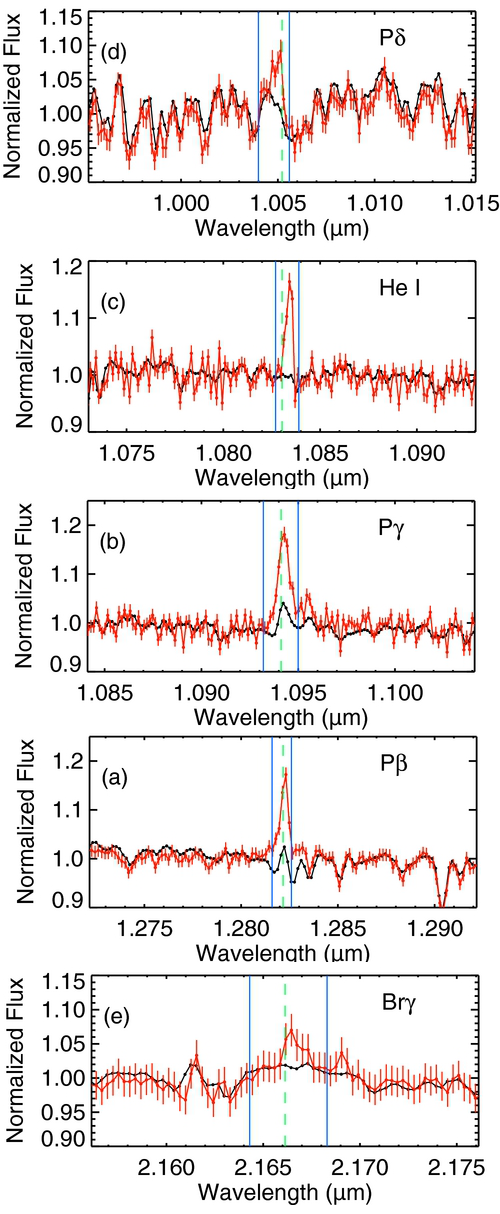
\includegraphics[width=\textwidth,height=0.95\textheight,keepaspectratio]{Flare2.png}
    \caption{Regions of the spectrum of EV Lac in and out of flare. A quiescent (non flaring) spectrum is shown in black and a spectrum taken while the star was flaring is in red. Source: \citet{2012Schmidt}.}
    \label{figFlareDia}
\end{figure}

\subsubsection{Influence of variability on exoplanet detection methods}
\label{secVarInfluence}
The timescale of these changes to the stellar surface will vary from minutes to days, depending on the mechanism producing them. Short duration variation will produce the low level, short period, signals seen in a periodogram like Figure\,\ref{figHD85512Power}. Longer duration variation may correspond to periodicities that can be falsely attributed to a potential exoplanet. For example, Kapetyn's star (GJ191) was observed by the HARPS team in 2014 and they reported two planets with periods of 48.6 and 121.5 days \citep{2014Anglada-Escude}. Further analysis by \citet{2015Robertson} found that the 48.6 day planet was most likely periodic magnetic activity causing a false radial velocity signal.\\

An individual convective granule is expected to add 1-2~kms$^{-1}$ of jitter; however, the fluctuations from the granules obey Poisson statistics and so the total radial velocity contribution by granules is dependent on the square root of the number of granules. The Sun has roughly 1 million granules visible at any one time, so the radial velocity noise from convective granulation scales down to 1-2~ms$^{-1}$ \citep{2003Lindegren}. Convective granules can last from minutes up to an hour, depending on size. Therefore \citet{2008Otoole} proposed that the simplest way to mitigate convective granulation jitter was to take several observations over the same night and take a mean spectrum, which would average out the fluctuations.\\

Pressure mode stellar oscillations will stretch and compress the plasma they travel through on timescales of 5 to 15 minutes \citep{2000Schrijver}. This will introduce a jitter of 0.01-0.4 ms$^{-1}$ into any radial velocity measurements, depending on the class of star. The amplitude of the jitter was found to be related to the luminosity/mass ratio \citep{2004Christensen-Dalsgaard}, so for cool stars like M-dwarfs, the jitter will be at the lower end of this range. By setting a minimum exposure time of 15 minutes, \citet{2011Dumusque} proposed that the radial velocity influence of the oscillations would be avoided.\\ 

M-dwarfs are known to be quite active, with starspots as a significant source of jitter. The light we observe comes from the whole visible face of the star. As the star is rotating, the light from the side rotating towards us will be blueshifted, and the light from the side rotating away will be redshifted. However, when a starspot rotates into view, the light from the blueshifted side will be reduced due to the spot-affected area being cooler than its surroundings. This imbalance in the amount of light coming from each side will also break the symmetry of a line profile. This effect is illustrated in Figure\,\ref{figSpotRotation}. Initially the starspot is not visible and the profile of the spectral line is symmetrical. As the starspot rotates into view, it suppresses some of the blueshifted flux, changing the profile of the blue side of the line and producing an asymmetry. Once it is directly in our field of view the symmetry is restored, but only because the flux is suppressed evenly across both sides of the line, producing a weaker, but symmetrical line. Once the spot begins to rotate away from view, the redshifted light is suppressed. Starspots on the Sun, which is considered to be somewhat quiescent compared to other main-sequence dwarfs, have been found to add around 0.65 ms$^{-1}$ of jitter \citep{2009Makarov}. The magnitude of this jitter is expected to be greater for more active stars such as M-dwarfs, and for faster rotating stars.\\

\begin{figure}
    \centering
    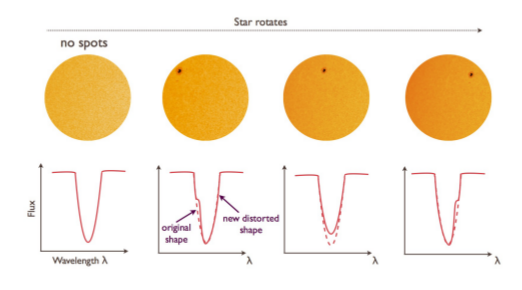
\includegraphics[width=0.8\textwidth]{SpotRotation.png}
    \caption{As a starspot rotates into view, it will first block the blueshifted side of the star, then cross the face to the redshifted side before moving out of view. Source: \citet{2015Haywood}.}
    \label{figSpotRotation}
\end{figure}

Faculae and plages affect the plasma of the star in a similar manner to starspots. While their influence on the temperature of the plasma is not as strong, they are spread out over a much larger area. Models of the Sun by \citet{2010Meunier} indicate that plages will add 8-10~ms$^{-1}$ of jitter, and a study of 171 G, K, and M stars by \citet{2020Hojjatpanah} found jitter on similar scales for faculae.\\

As the CCF is based of the profile of lines in a spectrum, the sudden increase in strength of select emission lines from flares will impact the CCF and therefore the radial velocity. The jitter produced will on the order of tens of ms$^{-1}$ \citep{2009Reiners}. However, flares occur sporadically and have timescales of minutes, so a it is unlikely for more than a single observation to capture flaring activity. Emission in the core of the H$\alpha$ line is particularly sensitive to flares, making it a useful tool to identify and removed affected observations.\\

While strong chromospheric and photometric activity in stars are known to produce detectable radial velocity variations, work by \citealt{2014Bastien} found measurable radial velocity variations in chromospherically and photometrically quiescent stars. They combined transit photometry from the Kepler survey, and spectra from the California Planet Search\footnote{$http://exoplanets.org/exoplanets_pub.html$} for 12 stars with low S-index measurements (see Section\ref{secVarQuant} for details on S-indices). For each star, radial velocities were measured for all spectra and the standard deviation across 2-hour bins was determined. They found radial velocity variations of several ms$^{-1}$, with one star varying by almost 136\,ms$^{-1}$! Further analysis found that the radial velocity variations strongly correlated with the number of significant peaks in the Fourier power spectrum of the photometric variability (where `significant' means the strongest peak and all peaks with a power \textgreater10\% of the strongest peak). They suggested that faculae might dominate in slowly rotating stars, producing low photometric activity, but more significant radial velocity variations.
\subsubsection{Quantifying the impact of variability}
\label{secVarQuant}
Any radial velocity measurement taken from a spectrum will include contributions from jitter. The greater the amount of jitter, the further away any single measurement of the RV can be from the ``true'' velocity, and the harder it will be to determine small amplitude periodic variations in radial velocity. While some jitter can be mitigated by the choice of suitably long exposure times and other observing strategy choices, other jitter mechanisms are unavoidable. Some stars will have moderate to low levels of activity that have little influence on the quantities we are trying to measure, while other stars will be so strongly affected by variability that the precision of radial velocity measurements required to detect an exoplanet above the noise will be impossible. Identifying these stars is important so that optimal observing targets can be prioritised. Metrics that can predict the variability of a star are valuable tools. \\

\begin{figure}
    \centering
    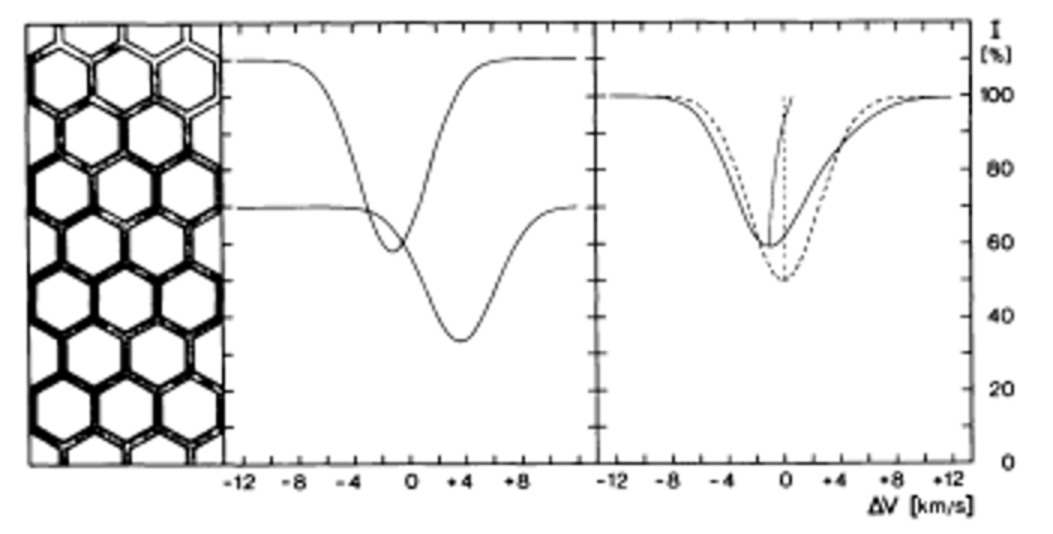
\includegraphics[width=0.8\textwidth]{LPV_convection.pdf}
    \caption{Schematic illustration of how convective granules affect the profile of spectral lines. Source: \citet{1981Dravins}.}
    \label{figLineProfile}
\end{figure}

An idealistic view of a stellar spectral line could be thought of as Lorentzian and symmetric. However, processes like convection will break that symmetry. \citet{1981Dravins} modelled the effect of granulation on the profile of a spectral line and Figure\,\ref{figLineProfile} is an example. The left panel is a diagram of the convective granules and the intergranular lanes. Their model assumed that 75\% of the visible face of the star was covered with granules, with an upward flow in the granules moving at 1.2 kms$^{-1}$ and the downward flow in the intergranular lanes moving at 3.6 kms$^{-1}$. Each of these flows produces a different line profile in the centre panel, with the stronger and bluer profile produced by the granules, and the weaker and redder profile coming from the intergranular lanes. The solid line in the right panel is the sum of both of these profiles, while the dashed line is the profile if there were no interference from granulation. Comparing the two profiles, it is obvious that the profile affected by convection is asymmetrical and bluer when compared to the unaffected profile. Changes to the line asymmetry over time will produce changes in the radial velocity over the same timescale. As the CCF represents the average line shape in the spectrum, measuring the change in the shape of the CCF over time is a useful metric of stellar activity.\\

\begin{figure}
    \centering
    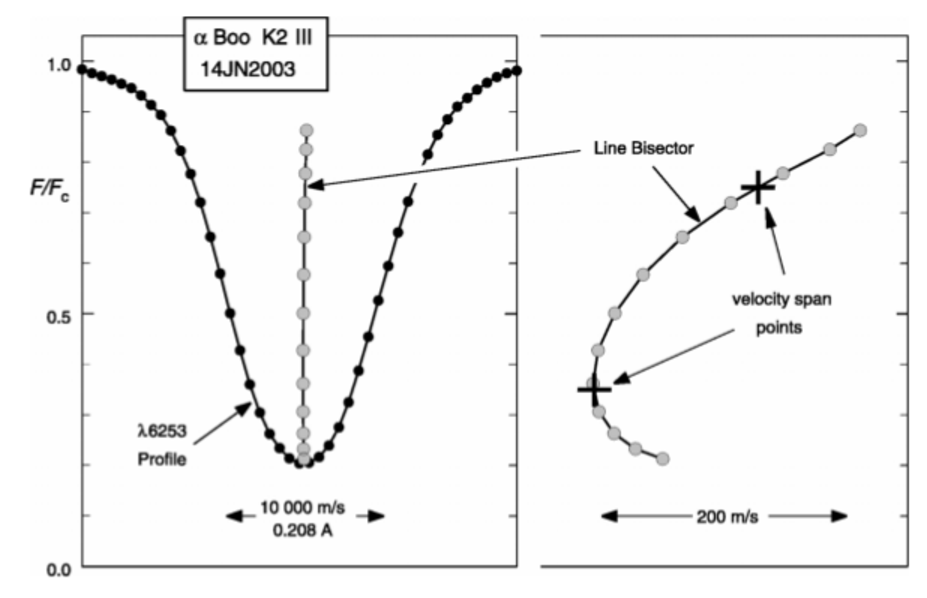
\includegraphics[width=0.8\textwidth]{Bisector.pdf}
    \caption{Line profile and bisector of the Fe line at 6253\,\AA\: in the spectrum of Arcturus. The right panel is zoomed in on the line bisector. Source: \citet{2006Gray}.}
    \label{figBis}
\end{figure}

Another tool for quantifying variability is the line bisector. If we were to sample a line in wavelength space, or a CCF in velocity space, at multiple points along the y-axis (the points in Figure\,\ref{figBis}) and obtain the the horizontal mid-point at each point (the grey points in the figure), then the trend of these mid-points would carry information about the shape of the line, and therefore about the levels of activity present. For a perfectly quiet star, we could assume that the bisector would be vertical; however, the convective granulation that produced the asymmetrical line profile will result in a curved bisector, seen in the right panel of Figure\,\ref{figBis}. There are multiple ways of using the bisector, including the bisector velocity span \citep{1988Toner} and the Bisector Inverse Slope (BIS) of the CCF \citep{2001Queloz}. If the bisector is determined across multiple observations, these methods can provide a measure of how the surface of the star is changing over time that can be correlated with radial velocity to determine whether the periodic changes of a specific period are due to stellar activity.\\

\begin{figure}
    \captionsetup{width=.8\textwidth}
    \subfloat[]{\label{figNaDfull}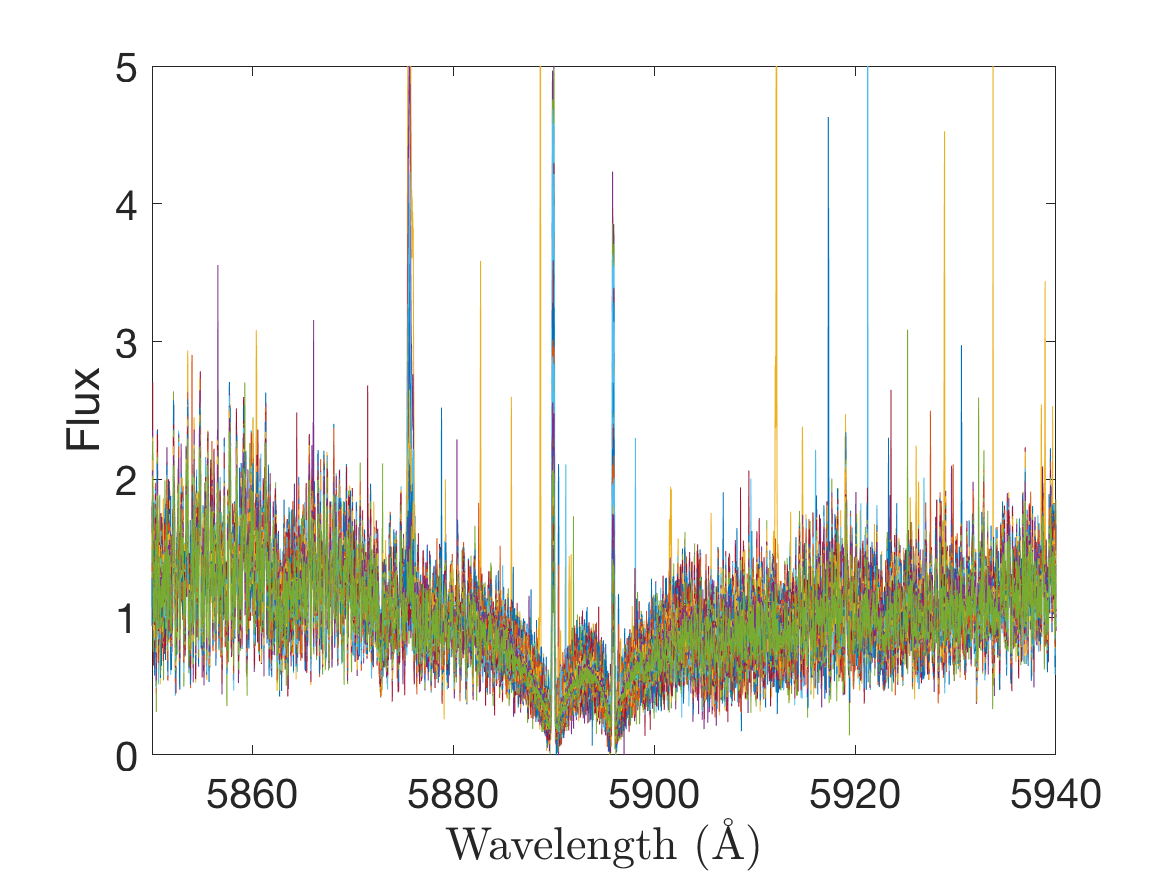
\includegraphics[width=0.5\textwidth]{NaDfull.png}}
    \subfloat[]{\label{figNaDzoom}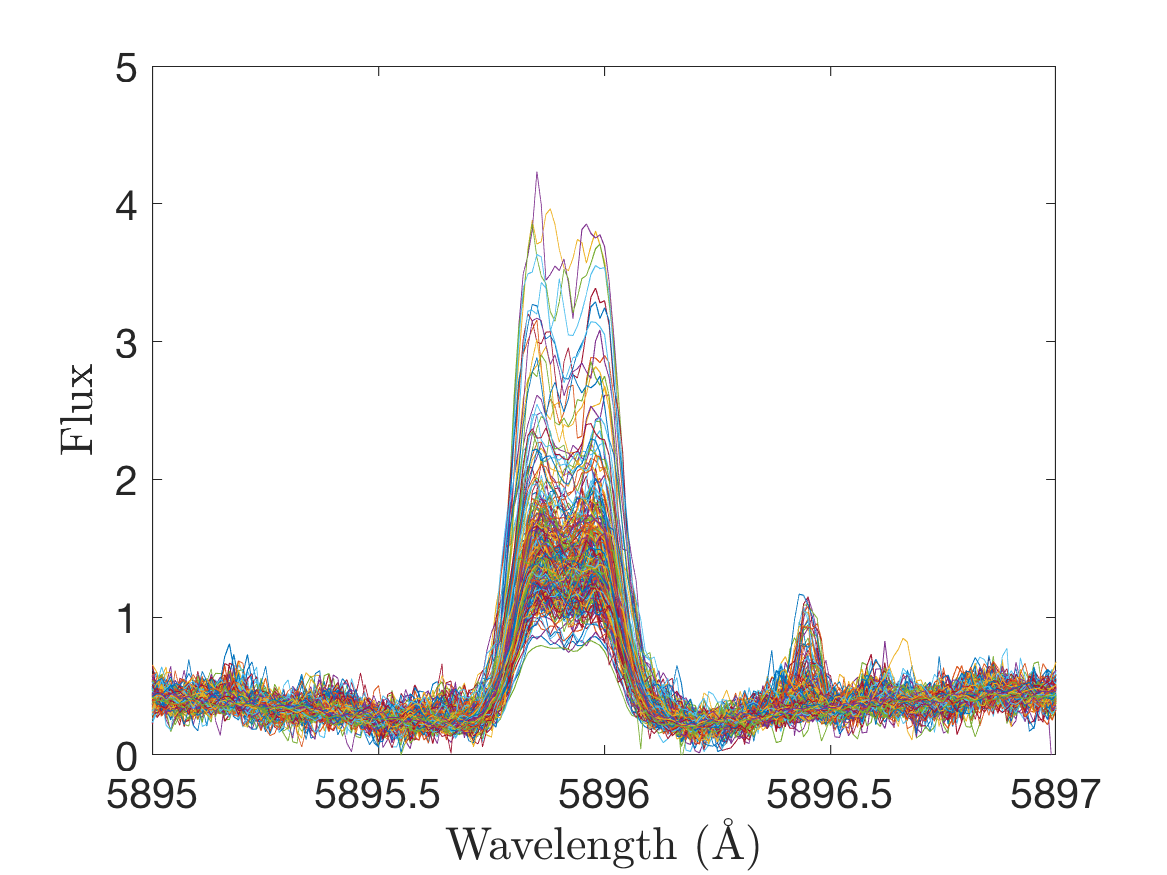
\includegraphics[width=0.5\textwidth]{Gl551_NaD_example.png}}
    \caption{Continuum normalised HARPS Spectra of GL551, focusing on one of the Na\,\textsc{i} D lines. In the core of the absorption line are two emission features that vary from observation to observation.}
    \label{figNaD_line}
\end{figure}

A stellar atmosphere will produce absorption and emission features in the spectrum of the star. Changes to the structure of the atmosphere will result in a change to the features in the spectrum, and therefore a change to any radial velocity measurement that uses those features. Several strong absorption lines have emission features at their cores that vary in strength over time, and the magnitude of this change correlates with changes in the radial velocity of the star. The most commonly used lines are Ca\,\textsc{ii} H (3968.47\,\AA) \& K (3933.66\,\AA), H\,\textsc{$\alpha$} (6562.808\,\AA), and Na\,\textsc{i} D doublet (5889.95\,\AA \& 5895.92\,\AA). An example of this is Figure\,\ref{figNaD_line} in which a Na\,\textsc{i} D emission feature can be clearly seen to vary in strength over a number of observations.\\

\begin{figure}
    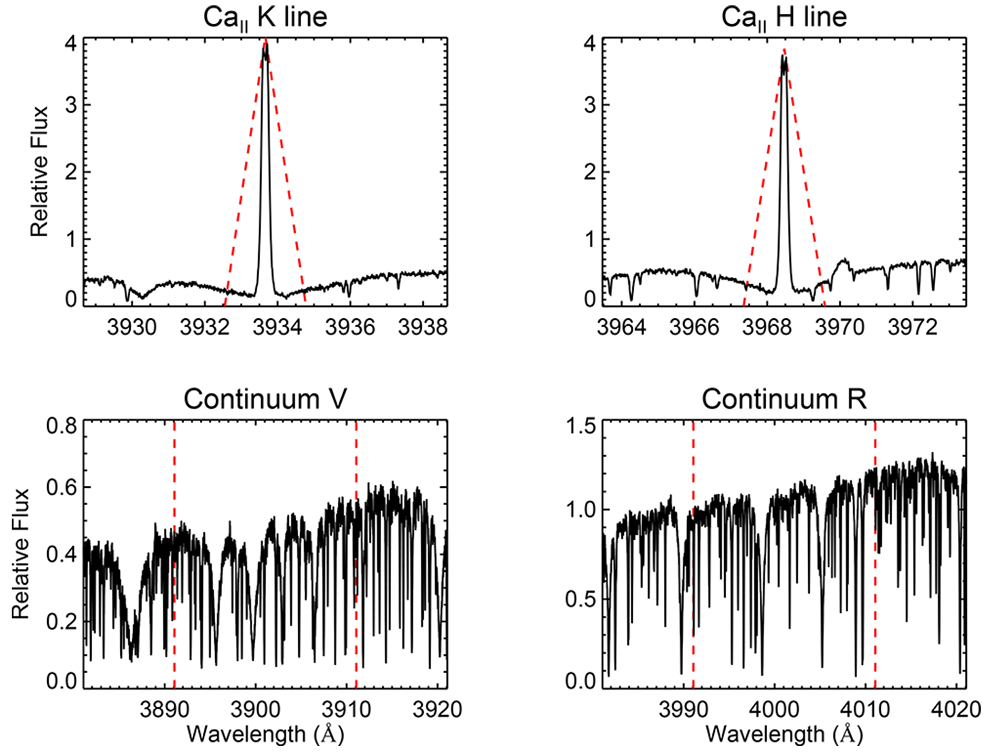
\includegraphics[scale=0.5]{MtWilson.png}
    \caption{Small regions of the spectrum of GJ176, with red dashed lines indicating the bandpasses for the Mount Wilson S-index (Equation\,\ref{eqSind}). The upper panels show the K and H feature bands, and the lower panels show the violet and red sidebands. Source: \citet{2015Suarez}.}
    \label{figLPVexample}
\end{figure}

The Ca\,\textsc{ii} H \& K lines are useful as they are strong and are in the visible wavelength range. The absorption comes from the photosphere, while the emission at the core of the line is produced in the upper photosphere and lower chromosphere, making it an excellent probe of those regions. \citet{1968Wilson} first correlated flux across the Ca\,\textsc{ii} H \& K lines to chromospheric activity by looking at the spectra of 91 main sequence stars over a roughly 10 year period. The product of this work was the Mount Wilson S-index (Equation \ref{eqSind}; \citealt{1978Vaughan}) which uses the flux in 1\,\hbox{\AA} passbands across each of the Ca\,\textsc{ii} H \& K lines. To normalise the measurement, they took the flux, $f(\lambda)d\lambda$, from 25\,\hbox{\AA} sidebands on the violet and red sides of the two calcium lines. Figure\,\ref{figLPVexample} displays the regions containing the passbands and sidebands used in the S-index. Since that time different groups have adapted the wavelength regions to better suit the type of star they are looking at or to refine the selection of the emission feature. For example, \citet{2011Gomes} decreased the line bandpass from 1\,\AA\:to 0.6\,\hbox{\AA} to exclude the line wings, which contain flux from the photosphere, and shifted to 20\,\hbox{\AA} sidebands centred around 3900\,\hbox{\AA} and 4000\,\hbox{\AA}.\\

\begin{equation}
	S_{HK} = \alpha\frac{\int_{3933.36}^{3933.96}f(\lambda)d\lambda+\int_{3968.17}^{3968.77}f(\lambda)d\lambda}{\int_{3890}^{3910}f(\lambda)d\lambda+\int_{3990}^{4010}f(\lambda)d\lambda}
	\label{eqSind}
\end{equation}

One issue with the S-index is that the values obtained are specific to the instrument and spectral type of the star. As such, a normalisation factor $\alpha$, based on observations of standard stars taken on the same night as the observation, is used to remove this dependence. See \citet{1982Middelkoop} for details of the normalisation factor. An alternative index that is independent of instrument and spectral class, $R^{\prime}_{HK}$, was developed by \citet{1984Noyes}. The main advantage of the $R^{\prime}_{HK}$ index (Equation\,\ref{eqRind}) over the S-index is that it measures activity in the lower chromosphere only, unlike the S-index which measures activity in both the upper photosphere and lower chromosphere. This is achieved by measuring the flux across the H and K lines as per the S-index, subtracting the photospheric flux from a quiescent reference star, leaving only the chromospheric flux $f^{\prime}(\lambda)d\lambda$, and replacing the denominator with $\sigma T^{4}$. The logarithm of this index is often reported as log($R^{\prime}_{HK}$).\\

\begin{equation}
	R^{\prime}_{HK} = \frac{\int_{3933.36}^{3933.96}f^{\prime}(\lambda)d\lambda+\int_{3968.07}^{3968.77}f^{\prime}(\lambda)d\lambda}{\sigma T^4_{eff}}
	\label{eqRind}
\end{equation}

These indices are commonly used to quantify chromospheric activity across most stars, however cool stars have insufficient flux in the Ca\,\textsc{ii} H \& K lines for $S_{HK}$ or log($R^{\prime}_{HK}$) to be a reliable proxy of stellar activity. Other chromospheric emission lines provide suitable replacement proxies of variability, such as H\,\textsc{$\alpha$} and the Na\,\textsc{i} D lines. H\,\textsc{$\alpha$} is located at the red end of the visible range and is sensitive to activity in the upper chromosphere. \citet{2014Gomes} investigated how useful S$_{H\alpha}$ was as an indicator of long period activity and found that S$_{H\alpha}$ correlated poorly with log($R^{\prime}_{HK}$) for stars with long period activity seen in log($R^{\prime}_{HK}$). The Na\,\textsc{i} D lines pair well with H\,\textsc{$\alpha$} because they all probe the lower to middle chromosphere \citep{2000Mauas}, allowing for full coverage of the chromosphere when both S$_{CaHK}$ and S$_{NaD}$ are determined.\\

\subsubsection{Application of variability indicators to spectroscopic data}
\label{secVarApp}
Once a periodic variation in the radial velocity is detected, the next step is to check that it is not the result of stellar activity. If changes in the radial velocity over time correlate with any of the variability measurements discussed in Section\,\ref{secVarQuant}, then it is highly likely that the periodic radial velocity signal comes from activity and not an exoplanet. For example, Figure\,\ref{figGL433_activity} shows that the radial velocity variations of GL433 (bottom panel) follow a similar pattern over time to an index measuring Na\,\textsc{i} D emission (middle panel). The two quantities have a Pearson coefficient of 0.91, indicating that they are highly correlated and the 1758.09 day period is most likely to be the result of long-term activity.\\

\begin{figure}
    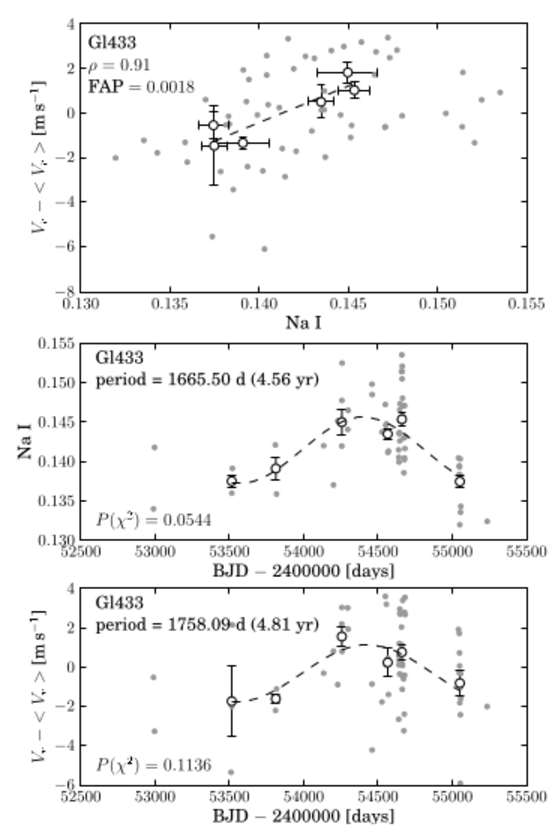
\includegraphics[width=0.8\textwidth]{Gl433_activity.pdf}
    \caption{Radial velocity and Na\,\textsc{i} D index measurements for GL433 (lower panels) and the correlation between the two (top panel). Source: \citet{2012Gomes}.}
    \label{figGL433_activity}
\end{figure}

Additionally, variability measurements can be analysed in parallel with the radial velocities. Taking the example of HD85512 from Section\,\ref{secRVanalysis}, the log($R^{\prime}_{HK}$) and BIS were measured for each observation and the periodograms for those quantities are shown in the middle and bottom panels of Figure\,\ref{figHD85512Periodogram}. There are peaks of significance at 58, 69, 85, and 300 days in the radial velocity panel, but the strengths of these peaks changes in the other two panels. The 300 day peak is the only one to have significant strength in all three measurements. Since the log($R^{\prime}_{HK}$) and BIS measurements are proxies for variability, the 300 day radial velocity peak is more likely to be the product of variability than a planet.\\

\begin{figure}
    \centering
    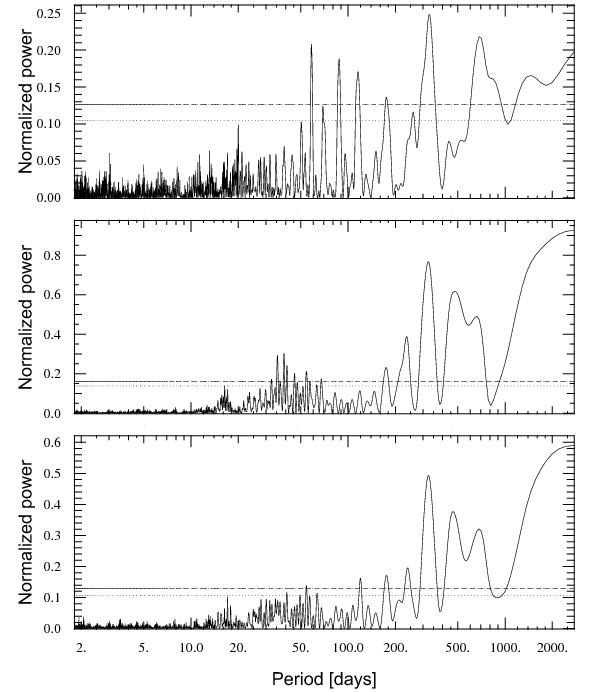
\includegraphics[width=0.8\textwidth]{HD85512_Periodogram.jpg}
    \caption{Periodograms of HD85512 produced from the (top) radial velocity, (middle) log($R^{\prime}_{HK}$), (bottom) line bisector BIS. Peaks at 58, 69, 85, and 300 days are found to be significant in the radial velocity measurements, and the 300 day period is also strong in the log($R^{\prime}_{HK}$) and BIS measurements. Dotted and dashed horizontal lines indicate FAP of 1\% and 10\% respectively. Source: \citet{2011Pepe}}
    \label{figHD85512Periodogram}
\end{figure}

\subsubsection{Radial velocity spectrographs}
\label{secSpecSurveys}
Exoplanet-focused spectroscopic surveys obtain multiple spectra of a sample of stars over a long enough time period to measure velocities over an orbit, although multiple orbits are preferable. These velocities are then analysed to look for periodic signals indicating the potential presence of exoplanets around the star. Detecting \textless1 ms$^{-1}$ radial velocities requires spectrographs built with high resolution (\textgreater 80,000) and intrinsic stability in mind. Two recent examples of exoplanet-focused spectrographs are HARPS and ESPRESSO.\\

Some of the most accurate radial velocities in recent time have come from the European Southern Observatory (ESO) High Accuracy Radial velocity Planet Searcher (HARPS; \citealt{2003Mayor}) spectrograph using the 3.6m telescope at La Silla, Chile. HARPS is a fibre-fed, cross-dispersed echelle spectrograph that was designed to be highly stable, allowing for radial velocities with precision of down to 1ms$^{-1}$. The spectrograph is placed inside a vacuum chamber which reduces the amount of spectroscopic line drift from atmospheric pressure changes to less than 0.1 ms$^{-1}$ \citep{2004Rupprecht}. Additionally, the temperature of the chamber is kept stable to 0.01\,K, and simultaneous Thorium-Argon wavelength calibration is used. The HARPS spectrograph has been used for multiple observing campaigns and has resulted in the detection of many exoplanets. Some highlights include the detection of a 1.7\,M$_\oplus$ exoplanet around GL581 \citep{2009Mayor}, one of the smallest detected exoplanets at the time, and a \textgreater1.2\,M$_\oplus$ exoplanet around Proxima Centauri \citep{2016AngladaEscude}, a star which is known to be active, making a confident detection of a planet difficult.\\

The Echelle Spectrograph for Rocky Exoplanet - and Stable Spectroscopic Observations (ESPRESSO; \citealt{2013Pepe}) is the successor to HARPS and saw first light in September 2016. It is a high-resolution (R $\sim$200,000), ultra-stable spectrograph with a wavelength coverage of 380\,-\,686 nm, and is installed on the Very Large Telescope (VLT). Due to the four 8.2 m telescopes comprising the VLT array, and improvements in laser-comb technology, ESPRESSO targets a precision of 30 cms$^{-1}$, a substantial improvement on HARPS. One of the significant results from ESPRESSO so far is the confirmation of a exoplanet around Proxima Centauri. \citet{2016AngladaEscude} found a 1.3 M$_\oplus$ exoplanet orbiting Proxima Centauri using radial velocities from HARPS and UVES\,\citep{2000Dekker} spectra. As Proxima Centauri is known to be very active, follow-up observations were required to confirm this detection as more data points allow for a better sampling of the orbit. The ESPRESSO data found the mass to be 1.29\,$\pm$\,0.13 M$_\oplus$ and the orbital period to be 11.218\,$\pm$\,0.029 days.

\section{Surveys relevant to this work}
\label{secSurvey}
There are multiple large-scale spectroscopic and photometric surveys that, while not specifically focused on exoplanets, have been used in the research presented in this thesis. Their key parameters are summarised here.\\

The Two Micron All Sky Survey (2MASS; \citealt{2006Skrutskie}) was a ground-based, full-sky photometric survey that used two 1.3 m telescopes, one in Chile and the other in Arizona, USA to obtain photometry of 470 million objects from 1997 to 2001. One of the major 2MASS data products was a point source catalogue that gives a comprehensive photometric view of stars in the Milky Way. 2MASS obtained photometry in the infrared J, H and K$_s$ passbands (1.2, 1.7 and 2.2\,$\mu$m).\\

The Wide-field Infrared Survey Explorer \citep[WISE;][]{2010Wright} is a satellite that was built by NASA to survey the whole sky at $3.4, 4.6, 12$ and $22 \mu m$ (W1, W2, W3, W4). The four WISE passbands are designed to be sensitive to emissions from different types of objects in the sky. M-dwarfs radiate sufficient flux across the wavelengths covered by W1 and W2 for these passbands to provide useful information. However, W3 and W4 occur at very red wavelengths, with insufficient flux to provide information about M-dwarf characteristics. Over 7 months in 2010, the WISE satellite obtained photometry of over 563 million objects. The full data set includes basic position information, photometric magnitudes for W1, W2, W3 and W4, and where possible, cross-matched J, H, and K$_s$ magnitudes from 2MASS.\\

\textit{Gaia} \citep{2016Gaia} is a space telescope and the successor to the HIgh Precision PARallax COllecting Satellite \citep[HIPPARCOS;][]{1981Kovalevsky} satellite. Its primary mission is to obtain photometry and a 5-component astrometric solution (right ascension, declination, proper motions, and parallax) for approximately 1 billion objects over a 5 year mission (2014-2019). In 2018 the \textit{Gaia} mission was assessed and was approved for an extension for as long as its on-board fuel lasts, which is predicted to be into 2024 \citep{2019Brown}. \textit{Gaia} will typically acquire 70 observations of each star during its operational phase, with the precision in the derived quantities increasing along with the volume of data. \textit{Gaia} collects photometry in a broad optical G passband and in narrower Bp and Rp filters. The precise and frequent astrometric measurements mean that highly accurate parallaxes and proper motions can be measured for most, if not all, of the stars it observes. Parallaxes are expected to be obtained with a precision of 9-11\,$\mu$as for stars brighter than V = 10, 10-27\,$\mu$as at V = 15, and 100-350\,$\mu$as at V = 20. \textit{Gaia} also collects objective prism spectra and determines radial velocities for stars brighter than V = 15 with an accuracy of between 1\,-\,15\,kms$^{-1}$.\\

The GALactic Archaeology with HERMES (GALAH) survey \citep{2021Buder} is a high-resolution (R\,=\,28,000), multi-object spectroscopic survey that is observing 1 million Milky Way stars using the High Efficiency and Resolution Multi Element Spectrograph (HERMES) spectrograph \citep{2015Sheinis}. The aim of the survey is to study the history of star formation, chemical enrichment, and minor mergers in the Milky Way. Because this requires detailed chemical abundance measurements, the HERMES cameras cover four wavelength regions that deliver information on stellar parameters and 30 different elements from all major nucleosynthetic channels. The bandpasses are blue (4718-4903$\hbox{\AA}$); green (5649-5873$\hbox{\AA}$); red (6481-6739$\hbox{\AA}$) and infrared (7590-7890$\hbox{\AA}$). The spectra are reduced in a pipeline described by \citet{2017Kos} and analysed using Spectroscopy Made Easy \citep[SME;][]{1996Valenti}. Chapter\,\ref{chapGALAH} details the use of M and K dwarf spectra from this survey to identify active spectral lines across the GALAH bandpasses and investigate the effect of that activity on abundance determination.

\section{Research motivation}
M-dwarfs are excellent candidates as hosts of small rocky planets orbiting in the habitable zone. There are a large number of absorption lines in their spectra, and they tend to rotate slowly, facilitating precise measurements of their radial velocities. Their habitable zones are located relatively close to the star, increasing the detectability of planets orbiting at those distances. But as mentioned previously, there are several obstacles to overcome:\\

Identifying an M-dwarf typically requires a spectrum. For a small sample of stars, obtaining this information is not a difficult task. However, for larger samples, especially for large surveys, this would require significant telescope time. A method by which we could identify M-dwarfs with minimal additional observations would be beneficial. This work, originally published in the Monthly Notices of the Royal Astronomical Society \citep{2019Bentley}, is explored in Chapter\,\ref{ChapPhot}.\\

Additionally, M-dwarfs are known to be very active early in their lifetimes. While active stars can provide useful information about how planets develop in extreme environments, high levels of stellar activity disrupt our ability to detect exoplanets through radial velocity, making them less useful for planet searches. So for efficiency, active stars will need to be identified and not observed further. Existing indices for the Ca\,\textsc{ii} H \& K, H\,\textsc{$\alpha$}, and Na\,\textsc{i} D features are known to correlate with stellar activity, but they are only useful if there is sufficient flux in the spectrum for at least one of these lines. An index that works across a broader range of wavelength would be more useful, especially if it used the same wavelength range we use to measure the radial velocity. Chapter\,\ref{chapISV} develops such a method.\\

Once these selection methods have been developed, they need to be tested on data from other surveys to see how well they translate. Additionally, a large sample of stars would provide an opportunity to investigate how the activity measured using the techniques of Chapter 3 presents in other classes of star. In this case, K- and M- dwarfs were identified in the GALAH survey using the selection method of Chapter 2, and the variability metric of Chapter 3 was applied to spectra of many stars in narrow ranges of absolute magnitude. The influence of stellar luminosity and the number of stars included on the measurement uncertainty of the variability metric, and the influence of variability of the precision of elemental abundances were investigated. The details are presented in Chapter\,\ref{chapGALAH}.